\documentclass[lettersize,journal]{IEEEtran}
\IEEEoverridecommandlockouts
% The preceding line is only needed to identify funding in the first footnote. If that is unneeded, please comment it out.
%Template version as of 6/27/2024
\hyphenation{op-tical net-works semi-conduc-tor IEEE-Xplore}
\def\BibTeX{{\rm B\kern-.05em{\sc i\kern-.025em b}\kern-.08em
    T\kern-.1667em\lower.7ex\hbox{E}\kern-.125emX}}
% The preceding line is only needed to identify funding in the first footnote. If that is unneeded, please comment it out.
\usepackage{float}
\usepackage{placeins}
\usepackage[caption=false,font=normalsize,labelfont=sf,textfont=sf]{subfig}
\usepackage{amsthm}
\usepackage{makecell}
\usepackage{cite}
\usepackage{multirow}
\usepackage{amsmath,amssymb,amsfonts}
% \usepackage{algorithmic}
\usepackage{graphicx}
\usepackage{textcomp}
\usepackage{xcolor}
\usepackage{enumerate}
\usepackage{framed}
\usepackage{subcaption}
\usepackage{url}
\usepackage{footnote}
\usepackage{tcolorbox}
\usepackage{epsfig,endnotes,amsfonts,bm,tikz,pgfplots}
\usepackage{indentfirst}
\usepackage{amssymb}
\usepackage{pifont}
\usepackage{epstopdf}
\usepackage{algorithm}
% \usepackage{algorithmic}
\usepackage{algpseudocode}
\usepackage{booktabs}
\newcommand{\cmark}{\ding{51}}%
\newcommand{\xmark}{\ding{55}}%






% hyperref is loaded with options below.
\usepackage[russian,english]{babel}
\usepackage{xcolor}
\usepackage{amssymb}% http://ctan.org/pkg/amssymb
\usepackage{pifont}% http://ctan.org/pkg/pifont
\usepackage{pgfplots}
\usepackage{pgfplotstable}
\usepgfplotslibrary{groupplots}
\pgfplotsset{compat=1.18}



\usepackage{tcolorbox}

\newtheorem{assumption}{Assumption}
\newtheorem{definition}{Definition}
\newtheorem{theorem}{Theorem}
\newtheorem{lemma}{Lemma}
\newtheorem{remark}{Remark}




\newcommand{\ZZ}{\mathbb{Z}}
\newcommand{\GG}{\mathbb{G}}
\newcommand{\FF}{\mathbb{F}}
\newcommand{\CompExp}{\mathcal{E}}
\newcommand{\CompPair}{\mathcal{P}}
\newcommand{\CompField}{\mathcal{F}}
\newcommand{\ComField}{\CompField}



\newcommand{\dleq}{\mathsf{DLEQ}}
\newcommand{\dleqvrf}{\mathsf{DLEQVrf}}


% 定义变量
% \newcommand{\ssshare}{\mathsf{SS.Share}}
% \newcommand{\ssrec}{\mathsf{SS.Reconstruct}}
\newcommand{\vssreshare}{\mathsf{VSS.ReShare}}
\newcommand{\vssaggregate}{\mathsf{VSS.ReshareAgg}}
\newcommand{\vssrerec}{\mathsf{VSS.ReshareRec}}


\newcommand{\vssshare}{\mathsf{VSS.Share}}
\newcommand{\vssvrf}{\mathsf{VSS.Verify}}
\newcommand{\vssrec}{\mathsf{VSS.Reconstruct}}

\newcommand{\DKGGenPK}{\mathsf{DKG.GenPK}}
\newcommand{\DKGGenSK}{\mathsf{DKG.GenSK}}

\newcommand{\blssetup}{\mathsf{BLS.Setup}}
\newcommand{\blskeygen}{\mathsf{BLS.KeyGen}}
\newcommand{\blssign}{\mathsf{BLS.Sign}}
\newcommand{\blsvrf}{\mathsf{BLS.Verify}}
\newcommand{\blscombine}{\mathsf{BLS.Combine}}
\newcommand{\blsbatch}{\mathsf{BLS.Batch}}
\newcommand{\blsbatchvrf}{\mathsf{BLS.BatchVrf}}

\newcommand{\pssetup}{\mathsf{PS.Setup}}
\newcommand{\pskeygen}{\mathsf{PS.Kengen}}
\newcommand{\psPrepareBlindSign}{\mathsf{PS.PrepareBlindSign}}
\newcommand{\psBlindSign}{\mathsf{PS.BlindSign}}
\newcommand{\psUnblind}{\mathsf{PS.Unblind}}
\newcommand{\psSign}{\mathsf{PS.Sign}}
\newcommand{\psobtaincred}{\mathsf{PS.ObtainCred}}
\newcommand{\psgentoken}{\mathsf{PS.GenToken}}
\newcommand{\psver}{\mathsf{PS.Verify}}


\newcommand{\dacsetup}{\mathsf{DAC.Setup}}
\newcommand{\dacevolve}{\mathsf{DAC.Evolve}}
\newcommand{\dackeygen}{\mathsf{DAC.Kengen}}
\newcommand{\dacPrepareBlindSign}{\mathsf{DAC.PrepareBlindSign}}
\newcommand{\dacBlindSign}{\mathsf{DAC.BlindSign}}
\newcommand{\dacobtaincred}{\mathsf{DAC.ObtainCred}}
\newcommand{\dacgentoken}{\mathsf{DAC.GenToken}}
\newcommand{\dacver}{\mathsf{DAC.VerifyTok}}
\newcommand{\dactrace}{\mathsf{DAC.Trace}}


\newcommand{\dacadd}{\mathsf{DAC.AddAttr}}
\newcommand{\dacupdate}{\mathsf{DAC.UpdateAttr}}
\newcommand{\dacremeove}{\mathsf{DAC.RemoveAttr}}
\newcommand{\dacquerry}{\mathsf{DAC.QueryAttr}}



\newcommand{\RDKGGenPK}{\mathsf{RDKG.GenPK}}
\newcommand{\RDKGEvolve}{\mathsf{RDKG.Evolve}}
\newcommand{\RDKGGenSK}{\mathsf{RDKG.GenSK}}

\newcommand{\SK}{\mathsf{SK}}
\newcommand{\PK}{\mathsf{PK}}
\newcommand{\PP}{\mathsf{PP}}


\newcommand{\SA}{\mathsf{SA}}
\newcommand{\SAGetPub}{\mathsf{SA.GetPub}}
\newcommand{\SAGetPriv}{\mathsf{SA.GetPriv}}
\newcommand{\SApk}{\mathbf{PK}}
\newcommand{\SAsk}{\mathbf{SK}}
\newcommand{\SAr}{\mathbf{R}}
% ---------- Math Packages ----------
\usepackage{amsmath,amssymb,amsfonts,amsthm}
\usepackage{bm}

% ---------- Fields and Groups ----------
\newcommand{\Fp}{\FF_p}
\newcommand{\GOne}{G_1}
\newcommand{\GTwo}{G_2}
\newcommand{\GT}{G_T}
\newcommand{\pair}{e}

% ---------- Structured Reference String ----------
\newcommand{\SRS}{\mathsf{SRS}}

% ---------- Hash Functions ----------
% \newcommand{\Hleaf}{H_{\mathsf{leaf}}}
% \newcommand{\Hnode}{H_{\mathsf{node}}}
% \newcommand{\Hfs}{H_{\mathsf{fs}}}
% \newcommand{\Hfsa}{H_2}
% \newcommand{\Hfsz}{H_2}

% ---------- Protocol Algorithms ----------
\newcommand{\Setup}{\mathsf{Setup}}
\newcommand{\Store}{\mathsf{Store}}
\newcommand{\Chal}{\mathsf{Challenge}}
\newcommand{\ProofGen}{\mathsf{ProofGen}}
\newcommand{\Verify}{\mathsf{Verify}}
\newcommand{\VerifyTagAuth}{\mathsf{VerifyTagAuth}}

% ---------- Common Objects ----------

\newcommand{\Auth}{\mathsf{Auth}}


% ---------- Commitment-Related Symbols ----------
\newcommand{\Cq}{C_q}
\newcommand{\Cqr}{C_{qr}}
\newcommand{\CF}{C_Q}
\newcommand{\RF}{R_Q}
\newcommand{\VF}{V_Q}
\newcommand{\VFt}{\widetilde{V}_Q}
\newcommand{\pibatch}{\pi_{\mathsf{batch}}}

% ---------- Optional Operators ----------
\DeclareMathOperator{\polydeg}{deg}




\definecolor{CitationBlue}{RGB}{0,76,153}
% \usepackage[colorlinks]{hyperref}
\usepackage[pdfstartview=FitH,
            bookmarksnumbered=true,
            bookmarksopen=true,
            colorlinks,
            pdfborder=001,   %注释掉此项则交叉引用为彩色边框
            linkcolor=blue,
            anchorcolor=blue,
            urlcolor=blue,
            citecolor=CitationBlue]{hyperref}
\hypersetup{
    colorlinks=true,
    citecolor=CitationBlue
}
\usepackage[
	lambda,
	advantage,
	operators,
	sets,
	adversary,
	landau,
	probability,
	notions,
% 	logic,
	ff,
	mm,
	primitives,
	events,
	complexity,
	asymptotics,
	keys
	]{cryptocode}

 \usepackage{tcolorbox}
\tcbuselibrary{skins, breakable}
\usepackage[
	lambda,
	advantage,
	operators,
	sets,
	adversary,
	landau,
	probability,
	notions,
% 	logic,
	ff,
	mm,
	primitives,
	events,
	complexity,
	asymptotics,
	keys
	]{cryptocode}
\createprocedurecommand{functionality}{}{\textbf{Functionality~}}{mode=text}

\newtcolorbox{functionality2}[2][]{
    colback = white,
    fonttitle = \sffamily\bfseries,
    colbacktitle = white,
    coltitle = black, enhanced,
    attach boxed title to top left = {xshift=12pt, yshift=-\tcboxedtitleheight/2},
    boxrule = 1 pt,
    top = \tcboxedtitleheight/2,
    % breakable,
    title=Functionality\ #2,#1}

\begin{document}


\title{FoldAudit: Secure Multi-File Data Integrity Auditing via Folded KZG Verification}

\markboth{Journal of \LaTeX\ Class Files,~Vol.~14, No.~8, August~2021}%
{Shell \MakeLowercase{\textit{et al.}}: A Sample Article Using IEEEtran.cls for IEEE Journals}

\author{Liang Zhang,~\IEEEmembership{Member,~IEEE}, Xuyan Wei, Borui Chen, Haibin Kan$^*$,~\IEEEmembership{Member,~IEEE,} and Jiheng Zhang$^*$
\thanks{Liang Zhang and Jiheng Zhang are with Department of Industrial Engineering and Decision Analytics, Hong Kong University of Science and Technology, Clear Water Bay, Kowloon, Hong Kong. (e-mail: scottzhang@ust.hk; jiheng@ust.hk)}
\thanks{Xuyan Wei is with School of Cyberspace Security (School of Cryptology), Hainan University, Haikou, 570228, China. (e-mail: wxy2@hainanedu.cn)}
\thanks{Borui Chen and Haibin Kan are with College of Computer Science and Artificial Intelligence, Fudan University, Shanghai 200433, China. Haibin Kan is also with Shanghai Engineering Research Center of Blockchain, Shanghai 200433, China and Shanghai Institute for Mathematics and Interdisciplinary Sciences, Shanghai, 200433, China.(e-mail: 23210240072@m.fudan.edu.cn; hbkan@fudan.edu.cn;)}

\thanks{This work was supported by the National Natural Science Foundation of China (Nos. 62302129 and 62272107), the Project of Shanghai Science and Technology (Grant No. 2024ZX01), the Project of the Yiwu Research Institute of Fudan University, Hainan Province Key R\&D plan project (No. ZDYF2024GXJS030) and the HK RGC General Research Fund (No. T32-615/24-R).}

% \markboth{Journal of \LaTeX\ Class Files,~Vol.~14, No.~8, August~2021}%
% {Shell \MakeLowercase{\textit{et al.}}: A Sample Article Using IEEEtran.cls for IEEE Journals}
\thanks{*Corresponding author}
}

\maketitle
\begin{abstract}
Provable data possession (PDP) enables lightweight integrity auditing for outsourced storage without retrieving the entire dataset. Multi-file integrity auditing is increasingly important in outsourced storage systems, where users often maintain many independently updated files and delegate verification to external auditors. Although PDP techniques achieve sublinear checking through random sampling and homomorphic aggregation, extending them to polynomial-commitment-based multi-file auditing introduces two subtle challenges: public audit transcripts may leak challenged evaluations, and linear proof aggregation may allow corrupted components from different files to cancel each other algebraically.
This paper presents FoldAudit, a secure multi-file auditing protocol that combines Merkle authentication, independent file-specific evaluation points, and polynomial folding. FoldAudit compresses multiple polynomial opening relations into a single verification equation while preserving per-file accountability. To protect evaluation privacy, FoldAudit masks each challenged evaluation with fresh additive randomness and proves correct mask formation using Schnorr proofs. The protocol also supports stateless file insertion and active audit-set removal, ensuring that updates affect only the corresponding file metadata rather than the entire batch. We prove that, once corrupted chunks are sampled, the folded polynomial relation has negligible soundness error. Implementation results and comparisons demonstrate that FoldAudit provides practical, scalable, privacy-preserving, and cancellation-resistant multi-file cloud storage auditing.
\end{abstract}

\begin{IEEEkeywords}
Provable Data Possession, Data Integrity Auditing, KZG Commitments, Multi-File Auditing
\end{IEEEkeywords}


% 云存储风险 → PDP 基本机制 → 多文件/批量审计需求 → 多项式承诺发展 → 现有问题：隐私泄漏与 cancellation attack → FoldAudit 方案与贡献。
\section{Introduction}


The exponential growth of global data generation has driven a paradigm shift toward decentralized and cloud-based storage architectures. By outsourcing data to remote storage providers, individuals and organizations significantly reduce local hardware maintenance costs while benefiting from elastic scalability, geographic redundancy, and high availability~\cite{Shah2007Auditing,Sookhak2015Survey}. However, this outsourcing model inherently relinquishes physical control over the stored assets, exposing them to multifaceted risks such as hardware degradation, silent data corruption, and economically motivated data deletion or compression by untrusted storage providers~\cite{Deswarte2004RIC,Schwarz2006Store}. To mitigate these threats and restore trust in distributed storage ecosystems, Provable Data Possession (PDP)~\cite{Ateniese2007PDP,Bowers2009HAIL,Stefanov2012Iris,Ateniese2011RDC} and Proofs of retrievability (PoR)~\cite{Juels2007POR,Le2023Porla} schemes have emerged as foundational cryptographic primitives. These protocols enable data owners or delegated auditors to efficiently verify the integrity of outsourced data without retrieving the entire dataset, thereby ensuring continuous data availability, regulatory compliance, and accountability in modern storage networks.

Recent advancements in cryptographic primitives have significantly optimized the efficiency and scalability of data integrity auditing. Among these, Polynomial Commitment Schemes (PCS), such as KZG~\cite{Kate2010KZG} and Boneh et al.~\cite{Boneh2020PCS} constructions, have been widely adopted in state-of-the-art PDP designs~\cite{YuTC25,ZhangTPDS23}. By encoding data blocks as coefficients of low-degree polynomials over a finite field, PCS enables compact, constant-size commitments and supports homomorphic aggregation of multiple block tags. This algebraic structure allows cloud servers to generate succinct proofs of possession through polynomial evaluation and quotient computation~\cite{Dumas2023VESPo,Yu2024EDASVIC}, while verifiers can validate correctness using a minimal number of cryptographic operations. Consequently, polynomial commitments have become the cornerstone of lightweight, publicly verifiable auditing frameworks, reducing communication bandwidth or storage overhead. 
% Their compatibility with structured reference strings (SRS) and efficient synthetic division algorithms further positions them as ideal candidates for large-scale storage verification.


Despite these cryptographic improvements, practical storage deployments frequently involve massive-scale data repositories comprising thousands of files~\cite{ZhangTPDS23,XuTIFS26}. Conventional PDP protocols process each file independently, requiring separate proof generation, transmission, and verification rounds for every audited dataset. This linear scaling introduces severe computational and economic bottlenecks, particularly in blockchain-assisted auditing systems~\cite{Shu2022BlockchainAudit,Cui2024PayPerProof,Xu2024BDACD}. As audit frequencies increase and batch sizes grow, the cumulative overhead of independent verifications rapidly degrades system throughput, inflates operational expenses, and strains verifier resources. Therefore, developing an efficient multi-file batch verification mechanism has become a critical research imperative for scalable storage. Existing multi-file PDP schemes mainly optimize aggregation efficiency, dynamic updates, searchable auditing, or decentralized deployment~\cite{XuTIFS26,ZhangTPDS23,MiaoSCIS2026}. However, they rarely treat cancellation attacks as an explicit design target, where algebraically aggregated corruptions from different files may offset one another and pass a batch verification equation.


Given the substantial size of individual files in real-world applications, auditing every data block is computationally prohibitive and economically unviable. To address this challenge, modern PDP and PoR schemes universally employ probabilistic sampling strategies~\cite{Ateniese2008Scalable,Shacham2008POR,Dodis2009POR,Le2023Porla}. During an audit round, the verifier randomly selects a subset of data blocks and assigns independent random coefficients to construct a linear combination of challenged sectors. This approach reduces the proof size and verification complexity from linear $O(n)$ to constant or logarithmic $O(c)$ with respect to the total number of blocks, where $c \ll n$ denotes the challenge size. By carefully calibrating the number of sampled blocks, auditors can achieve high detection probabilities for data corruption while maintaining minimal communication and computation overhead. The randomness of the challenge set ensures that malicious providers cannot precompute proofs or selectively store only frequently accessed blocks without facing a high risk of detection.

However, the introduction of probabilistic sampling and homomorphic aggregation introduces subtle yet critical privacy vulnerabilities~\cite{Wang2010PrivacyAudit}. 
In many existing batch auditing designs, challenge generation mechanisms, evaluation points, and masking techniques are either oversimplified or structurally coupled across files~\cite{ZhangTPDS23,XuTIFS26}. 
If challenge points are shared, folding weights are predictable, or masking values are reused, an honest-but-curious verifier can exploit the linear algebraic structure of aggregated evaluations. Through cross-round correlation analysis or linear system inversion on publicly disclosed challenge-response transcripts, adversaries may reconstruct underlying polynomial evaluations or even infer sensitive sector values. Such privacy leakage fundamentally contradicts the confidentiality requirements of modern cloud and decentralized storage, highlighting the necessity of integrating masking directly into the verification procedure~\cite{Wang2013TC,MiaoSCIS2026}.


To address these challenges, we propose \textbf{FoldAudit}, a batch-verifiable PDP scheme for efficient and secure multi-file auditing. FoldAudit introduces a layered algebraic folding architecture with three core mechanisms. First, it assigns independent per-file challenge points to isolate file-specific quotient relations and prevent cross-file cancellation. Second, it derives the folding scalar through the Fiat--Shamir transform after the proof statement is fixed, making batch aggregation unpredictable and bias-resistant. Third, it applies additive one-time masking to challenged evaluations and binds each mask to a public commitment together with a Schnorr proof of knowledge~\cite{Schnorr1991Sig}, enabling practical evaluation privacy while preserving verifiability. For dynamic file sets, FoldAudit maintains a separate Merkle root and tag collection for each file, so that adding or removing a file affects only its own authentication state rather than requiring global recomputation.


The main contributions of this work are summarized as follows.
\begin{itemize}
    \item We design \textbf{FoldAudit}, a PDP-oriented multi-file auditing protocol that combines per-file tags, Merkle-authenticated sampled tags, independent file-specific evaluation points, and Fiat--Shamir folding into a single batch verification relation. The construction supports file addition and active audit-set removal without rebuilding a global commitment over all surviving files.

    \item We provide a security analysis of the folded audit relation. The analysis separates sampling-based detection from algebraic batch soundness, proves a folded polynomial soundness error of at most $(m-1)/p+\mathsf{negl}(\lambda)$ for challenged corrupted data, and formalizes the evaluation-privacy condition induced by additive one-time masks and Schnorr mask proofs.

    \item We give a unified comparison with representative PDP and data auditing schemes. The comparison identifies whether existing schemes support native multi-file batching, independent evaluation points, evaluation privacy, dynamic operations, and resistance to cross-file cancellation, and derives computation and communication costs under a common notation.

    \item We implement FoldAudit and source-level reproductions of representative protocols, and evaluate them by end-to-end execution under controlled variations of file size, sector count, and batch size. Experimental evaluations show that FoldAudit achieves competitive proof-generation, verification, and audit overhead across varying file sizes, sector counts, and batch sizes. 
\end{itemize}

\section{Preliminaries}
\label{sec:preliminaries}

\subsection{Merkle Tree}
A Merkle tree is a hash-based vector commitment supporting membership authentication. Let $H_1:\{0,1\}^*\rightarrow\{0,1\}^{\lambda}$ be a hash function. For an indexed value \(X_j\), a domain-separated leaf can be written as
$L_j=H_1(\mathsf{leaf}\|j\|\mathsf{enc}(X_j)),$
where \(\mathsf{enc}(\cdot)\) is an injective encoding. Internal nodes use a separate domain label,
$
N=H_1(\mathsf{node}\|N_{\mathsf{left}}\|N_{\mathsf{right}}),
$
until a root \(\Gamma\) is obtained. A membership proof consists of the sibling nodes on the path to \(\Gamma\), and a balanced tree with \(n\) leaves gives paths of length \(\lceil\log_2 n\rceil\).

\begin{assumption}[Collision Resistance]\label{ass:hash}
The hash function \(H_1:\{0,1\}^*\rightarrow\{0,1\}^{\lambda}\) is collision-resistant. Namely, for every PPT adversary \(\mathcal{A}\), $
    \Pr\!\left[
    x\neq x' \land H_1(x)=H_1(x')
    : (x,x')\leftarrow\mathcal{A}(1^\lambda)
    \right]\le \mathsf{negl}(\lambda).
$
\end{assumption}

\subsection{Polynomial Basics}

Let $\FF_p$ be a finite field of prime order $p$, and let $\FF_p^{<d}[X]$ denote univariate polynomials over $\FF_p$ of degree less than $d$. All polynomial identities are over $\FF_p[X]$, and all group exponents are interpreted modulo $p$.

For $f(X)\in\FF_p[X]$ and $r,y\in\FF_p$, the polynomial remainder theorem implies $f(X)-y=(X-r)w(X)+(f(r)-y)$
for a unique quotient polynomial $w(X)$. Thus $(X-r)$ divides $f(X)-y$ if and only if $y=f(r)$; in that case, $\deg(w)\le \deg(f)-1$.

\begin{lemma}[Schwartz--Zippel]\label{lem:schwartz_zippel}
Let $P(X)\in\FF_p[X]$ be a non-zero polynomial of degree at most $d$. For uniformly sampled $\rho\leftarrow\FF_p$, we have
    $\Pr[P(\rho)=0]\le \frac{d}{p}.$
\end{lemma}

\begin{lemma}[Random Linear Folding]\label{lem:random_linear_folding}
Let $\Delta_1,\ldots,\Delta_m\in\FF_p$ be field elements that are fixed before $\rho$ is sampled. If at least one $\Delta_i$ is non-zero and $\rho\leftarrow\FF_p$ is uniform, then
$\Pr_\rho\!\left[\sum_{i=1}^m \rho^{i-1}\Delta_i=0\right]\le \frac{m-1}{p}.$
\end{lemma}
\begin{proof}
The folded error polynomial $P_\Delta(T)=\sum_{i=1}^m \Delta_iT^{i-1}$ is non-zero and has degree at most $m-1$. The claim follows immediately from Lemma~\ref{lem:schwartz_zippel}.
\end{proof}



\subsection{KZG Polynomial Commitments}
We use the KZG polynomial commitment scheme~\cite{Kate2010KZG} over bilinear groups $(\GG_1,\GG_2,\GG_T,e)$ of prime order $p$, with generators $g\in\GG_1$ and $h\in\GG_2$. For degree-$<d$ polynomials, the structured reference string (SRS) is
\(\SRS=(g,g^\tau,\ldots,g^{\tau^{d-1}},h,h^\tau)\).
For \(f(X)=\sum_{k=0}^{d-1}a_kX^k\), the commitment is
\[
    C_f=g^{f(\tau)}=\prod_{k=0}^{d-1}(g^{\tau^k})^{a_k}.
\]
To open \(C_f\) at \(r\) with value \(y=f(r)\), the prover sends \(\pi=g^{w(\tau)}\), where \(w(X)=(f(X)-y)/(X-r)\). The verifier checks
\[
    e(C_f g^{-y},h)\stackrel{?}{=}e(\pi,h^\tau h^{-r}),
\]
which follows from \(f(\tau)-y=(\tau-r)w(\tau)\).

\begin{assumption}[KZG Binding and Knowledge Soundness]\label{ass:kzg_soundness}
For the SRS degree bound \(q\), the \(q\)-SDH assumption holds. Equivalently for our use, KZG commitments are computationally evaluation-binding and knowledge-sound for degree-\(\le q\) polynomials.
\end{assumption}

\subsection{Schnorr Proofs of Knowledge}
Schnorr proofs~\cite{Schnorr1991Sig} give a standard proof of knowledge for discrete logarithms in a prime-order group. For a public element \(Y=g^x\), the prover samples \(a\leftarrow\FF_p\), sends \(A=g^a\), receives a challenge \(\chi\), and responds with \(z=a+\chi x\). The verifier accepts if
\[
    g^z \stackrel{?}{=} A Y^\chi .
\]
In the Fiat--Shamir form, the verifier challenge is derived as \(\chi=H_2(Y,A)\), with domain separation supplied by the surrounding protocol. Knowledge soundness follows from the usual rewinding argument: two accepting transcripts with the same \(A\) and distinct challenges reveal \(x=(z-z')/(\chi-\chi')\).

\begin{assumption}[Random Oracle]\label{ass:random_oracle}
The Fiat--Shamir hash \(H_2\) is modeled as a domain-separated random oracle.
\end{assumption}

\begin{assumption}[Schnorr Knowledge Soundness]\label{ass:schnorr_knowledge}
Fiat--Shamir Schnorr proofs are knowledge-sound in the random oracle model.
\end{assumption}

\begin{assumption}[Discrete Logarithm Hardness]\label{ass:discrete_log}
The discrete logarithm problem is hard in \(\GG_1\). That is, for every PPT adversary \(\mathcal{A}\), $
    \Pr\!\left[y'=y:
    y\leftarrow\FF_p,\; Y=g^y,\; y'\leftarrow\mathcal{A}(g,Y)
    \right]\le \mathsf{negl}(\lambda).$
\end{assumption}




\section{System Model and Security Model}


\subsection{System Model}
\paragraph{System Entities}
We consider a batch-verifiable Provable Data Possession (PDP) architecture comprising three entities: a Data Owner (DO), a Cloud Server (CS), and a Verifier (V).
\begin{itemize}
    \item \textbf{Data Owner}: The DO outsources a batch of $m$ files to the CS for long-term storage. To ensure data integrity without maintaining local copies, the DO delegates periodic auditing to the V.
    \item \textbf{Cloud Server}: The CS is modeled as untrusted and computationally bounded: it may delete, corrupt, or selectively withhold files or chunks to save storage or bandwidth. 
    \item \textbf{Verifier}: The V is honest-but-curious. It executes the auditing protocol faithfully but may attempt to infer sensitive information from audit transcripts.
\end{itemize}

\paragraph{File Representation}
A file is divided into multiple chunks, and each \textbf{chunk} can be represented through polynomial coefficients. Each coefficient is referred to as a \textbf{sector}.
Let $m$ denote the number of files in a single audit batch, $n$ the number of chunks per file, and $s$ the number of sectors per chunk. Namely, each chunk is parsed into $s$ field elements from $\FF_p$ and algebraically encoded as a polynomial of degree at most $s-1$:
$$
    f_{i,j}(X) = \sum_{k=0}^{s-1} m_{i,j,k} X^k, \quad i \in [m], \; j \in [n],
$$
where $m_{i,j,k}$ represents the $k$-th sector of the $j$-th chunk in file $i$. 
A \textbf{tag} is used to represent the \(j\)-th chunk through a KZG polynomial commitment, i.e., $\sigma_{i,j} =  g^{f_{i,j}(\tau)} \in \GG_1$. Further, tags of each file are organized into a Merkle tree to guarantee correct indexing and membership.

Table~\ref{tab:notation} collects the protocol-specific symbols used in the system model and construction.

\begin{table}[htbp]
\centering
\caption{Summary of Notation and System Parameters}
\label{tab:notation}
\begin{tabular}{@{} p{0.04\textwidth} p{0.42\textwidth} @{}}
\hline
\textbf{Symbol} & \textbf{Description} \\
\hline
$\lambda$ & Security parameter. \\
$p$ & Prime order of $\FF_p$ and $(\GG_1, \GG_2, \GG_T)$. \\
$\FF_p^{<d}[X]$ & Polynomials over $\FF_p$ with degree less than $d$. \\
$g, h$ & Public generators of $\GG_1$ and $\GG_2$, respectively. \\
$e(\cdot, \cdot)$ & Bilinear map $e: \GG_1 \times \GG_2 \to \GG_T$. \\
$\tau$ & Secret trapdoor used for the structured reference string. \\
$\SRS$ & Public parameters $(g, g^\tau, \dots, g^{\tau^{s-1}}, h, h^\tau)$ supporting polynomial degrees $< s$. \\
$H_1$ & Hash function for Merkle tree construction. \\
$H_2$ & Fiat--Shamir random oracle for challenge derivation. \\
$m, n, s, c$ & Number of files, chunks per file, sectors per chunk, and challenged chunks per file. \\
$[m]$ & Index set $\{1, 2, \dots, m\}$ for the audited file batch. \\
$\delta$ & Fraction of corrupted or missing chunks. \\
$i, j, k$ & Indices for files ($i \in [m]$), chunks ($j \in [n]$), and sectors ($k \in [s]$). \\
$m_{i,j,k}$ & $k$-th sector value of chunk $j$ in file $i$. \\
$f_{i,j}(X)$ & Polynomial encoding of chunk $j$ in file $i$: $f_{i,j}(X) = \sum_{k=0}^{s-1} m_{i,j,k} X^k$. \\
$\sigma_{i,j}$ & KZG homomorphic tag for $f_{i,j}(X)$: $\sigma_{i,j} = g^{f_{i,j}(\tau)} \in \GG_1$. \\
$L_{i,j}$ & Merkle leaf for tag $\sigma_{i,j}$. \\
$\Gamma_i$ & Root hash of the Merkle tree for file $i$. \\
$J$ & Challenged chunk index set, $J \subseteq [n]$ with $|J| = c$. \\
$v_{i,j}$ & Random coefficient for challenged chunk $j$ of file $i$. \\
$r_i$ & Random evaluation point for file $i$. \\
$f_i(X)$ & Aggregated polynomial for each file $i$. \\
$y_i$ & Evaluation claim for file $i$: $y_i = f_i(r_i)$. \\
$b_i$ & Commitment of polynomial $f_i(X)$: $b_i=g^{f_i(\tau)}$. \\
$\mu_i$ & Fresh additive mask for the per-file evaluation $y_i$. \\
$\tilde{y}_i$ & Masked evaluation: $\tilde{y}_i = y_i + \mu_i$. \\
$R_i,\Pi_R$ & Mask commitment $R_i = g^{\mu_i}$ and Schnorr proof for $\mu_i$. \\
$w_i(X)$ & Per-file quotient polynomial of $f_i(X)$: $w_i(X) = \frac{f_i(X) - y_i}{X - r_i}$. \\
$C_{w_i}$ & Commitment to the quotient polynomial: $C_{w_i}=g^{w_i(\tau)}$. \\
$\rho$ & Fiat--Shamir-derived folding scalar for batch verification. \\
$\mathsf{chal}$ & The challenge tuple. \\
$\pi$ & The audit proof. \\
\hline
\end{tabular}
\end{table}

\paragraph{Protocol Workflow}
The provable data possession scheme for multiple files operates through five polynomial-time algorithms:
\begin{itemize}
    \item $\Setup(\lambda) \to \mathsf{pp}$: Generates public parameters $\mathsf{pp}$, including bilinear group tuples $(\GG_1, \GG_2, \GG_T, e)$, generators $(g,h)$, an SRS for degree $s-1$, and cryptographic hash functions $H_1$ (for Merkle tree construction) and $H_2$ (for Fiat--Shamir transcript hashing).
    \item $\Store(\{F_i\}_{i=1}^m) \to (\mathsf{data}, \mathsf{meta})$: The DO encodes each chunk into $f_{i,j}(X)$, computes tags $\sigma_{i,j}$, constructs the indexed Merkle tree over $L_{i,j}=H_1(\mathsf{leaf}\|\mathsf{fid}_i\|j\|\mathsf{enc}(\sigma_{i,j}))$ to obtain the root hash $\Gamma_i$ for each file, and outsources $\{F_i, \{\sigma_{i,j}\}, \text{Merkle trees}\}$ to the CS. The DO securely records $\{\Gamma_i\}_{i=1}^m$ and shares them with the V.
    \item $\Chal(m,n,c) \to \mathsf{chal}$: The verifier samples a shared challenge index set $J \subseteq [n]$ with $|J| = c$, random aggregation coefficients $\{v_{i,j}\}_{i\in[m], j \in J} \leftarrow \FF_p$, and per-file evaluation points $\{r_i\}_{i=1}^m \leftarrow \FF_p$. The challenge is $\mathsf{chal} = (J, \{v_{i,j}\}_{i\in[m],j\in J}, \{r_i\}, \mathsf{nonce})$, where $\mathsf{nonce}$ is a random value to resist replay attacks.
    \item $\ProofGen(\mathsf{chal}, \mathsf{data}, \mathsf{meta}) \to \pi$: The CS aggregates challenged chunks $J$ and outputs the corresponding non-interactive proofs $\pi$.
    \item $\Verify(\mathsf{chal}, \pi, \{\Gamma_i\}, \mathsf{pp}) \to \{\mathsf{accept}, \mathsf{reject}\}$: The V validates the integrity of all files $[m]$ via the proofs $\pi$.
\end{itemize}


\subsection{Security Model}
\label{sec:security_model}
FoldAudit is a spot-checking PDP protocol. Its soundness statement concerns possession of the challenged aggregate data in an audit round and the probability that corrupted or unavailable challenged chunks are detected. 
It does not provide a PoR-style retrievability guarantee or prove that the entire outsourced file can be reconstructed from audit transcripts.
The security of the proposed FoldAudit is formalized through three core properties: correctness, soundness, and privacy.


\textbf{Correctness}: If all parties (DO, CS, and V) execute the protocol honestly according to the specified algorithms, the $\Verify$ algorithm outputs $\mathsf{accept}$ with probability $1$.

\textbf{Soundness}:
Let $\mathcal{A}$ be a probabilistic polynomial-time (PPT) adversary controlling the CS. $\mathcal{A}$ wins the soundness game if it can produce a proof $\pi$ that causes $\Verify$ to output $\mathsf{accept}$ for a challenge involving corrupted, modified, or unavailable data chunks with non-negligible probability. 

\textbf{Privacy against Honest-but-Curious Verifier}:
Given the public audit transcript and the generated proof $\pi$, a PPT verifier cannot recover challenged evaluations $\{y_i = f_i(r_i)\}_{i=1}^m$ beyond feasible candidate testing, provided these evaluations have sufficient entropy. Raw data sectors remain hidden under the discrete-log hardness of the published commitments and the secrecy of the KZG trapdoor.


\section{Proposed Scheme}


\subsection{Construction}

\begin{figure*}[t]
  \centering
  \includegraphics[width=0.95\textwidth]{figures/pdpflowchart.pdf}
  \caption{System Model and Audit Workflow of FoldAudit}
  \label{fig:system model flowchar}
\end{figure*}


\paragraph{\textbf{Setup}} 
The $\Setup$ algorithm initializes the cryptographic environment and publishes the system-wide public parameters $\mathsf{pp}$. It first generates a bilinear group tuple $(\GG_1, \GG_2, \GG_T, e)$ of prime order $p$, selects public generators $g \in \GG_1$ and $h \in \GG_2$, and samples a secret trapdoor $\tau \in \FF_p$. Using $\tau$, the algorithm constructs the structured reference string \(\SRS=(g,g^{\tau}, \dots, g^{\tau^{s-1}}, h, h^{\tau})\), which supports polynomial commitments of degree strictly less than $s$. Cryptographic hash functions are fixed: $H_1$ for Merkle tree construction, and $H_2$ for Fiat--Shamir transcript binding. Finally, $\mathsf{pp} = (\GG_1, \GG_2, \GG_T, e, p, g, h, \SRS, H_1, H_2)$ is published. Each DO initializes an independent trapdoor and SRS for its own file batch; the trapdoor is not disclosed to the CS or V, while the published SRS is used for proof generation and verification.
% This trusted setup ensures that all subsequent polynomial commitments are evaluation-binding and knowledge-sound under standard hardness assumptions.
\begin{algorithm}[h]
\caption{$\Setup$}
\begin{algorithmic}[1]
\Require security parameter $\lambda$
\Ensure public parameters $\mathsf{pp}$
\State Generate $(\GG_1,\GG_2,\GG_T,e,p,g,h)$ and $\SRS=\left(g,g^\tau,\ldots,g^{\tau^{s-1}},h,h^\tau\right)$.
\State Fix cryptographic hashes $H_1, H_2$.
\State Publish
$
\mathsf{pp}=(\GG_1,\GG_2,\GG_T,e,p,g,h,\SRS, H_1,H_2).
$
\end{algorithmic}
\end{algorithm}


\paragraph{\textbf{File Storage}}
The $\Store$ algorithm handles data preprocessing, cryptographic tagging, and metadata generation for outsourcing. For each file $F_i$ ($i \in [m]$), the Data Owner parses every chunk $j \in [n]$ into $s$ field elements and algebraically encodes them as a polynomial $f_{i,j}(X) = \sum_{k=0}^{s-1} m_{i,j,k} X^k$. A KZG homomorphic tag $\sigma_{i,j} = g^{f_{i,j}(\tau)} \in \GG_1$ is computed for each chunk, providing a compact cryptographic binding to the underlying data sectors. Since \(\tau\) is known to the DO, the tag is computed by evaluating \(f_{i,j}(\tau)\) over \(\FF_p\) and then performing one base exponentiation in \(\GG_1\). 
Then, each tag is encoded as a domain-separated Merkle leaf $L_{i,j}=H_1(\mathsf{leaf}\|\mathsf{fid}_i\|j\|\mathsf{enc}(\sigma_{i,j}))$, and the leaves are organized into a Merkle tree with root $\Gamma_i$. The tree roots $\{\Gamma_i\}$ are securely retained by the DO (and later shared with the Verifier), while the raw data and tags are outsourced to the CS.
% This structure guarantees both data integrity and index authenticity without requiring the DO to maintain local copies.

\begin{algorithm}[h]
\caption{$\Store$}
\label{alg:store}
\begin{algorithmic}[1]
\Require files $\{F_i\}_{i=1}^m$
\Ensure outsourced data, metadata
\For{$i=1$ to $m$}
  \For{$j=1$ to $n$}
    \State Parse chunk $j$ into $s$ sectors and form $f_{i,j}(X)$.
    \State Compute tag $\sigma_{i,j}=g^{f_{i,j}(\tau)}$.
    \State $L_{i,j}\gets H_1(\mathsf{leaf}\|\mathsf{fid}_i\|j\|\mathsf{enc}(\sigma_{i,j}))$.
  \EndFor
  \State Build the $i$th Merkle tree over leaves $\{L_{i,j}\}_{j=1}^n$.
  \State Obtain root $\Gamma_i$.
\EndFor
\State DO sends $(F_i,\{\sigma_{i,j}\})$ to CS and records $\{\Gamma_i\}$ for V.
\end{algorithmic}
\end{algorithm}

\paragraph{\textbf{Challenge Generation}}
The $\Chal$ algorithm initiates the audit by sampling a challenge tuple $\mathsf{chal} = (J, \{v_{i,j}\}_{i\in[m],j\in J}, \{r_i\}_{i=1}^m,\mathsf{nonce})$. An index set $J \subseteq [n]$ of size $c$ is selected and applied to every audited file. Independent coefficients $\{v_{i,j}\}$ are drawn uniformly from $\FF_p$ to randomize each file's linear aggregation and prevent targeted corruption. Independent per-file evaluation points $\{r_i\}$ are sampled to support file-specific quotient checks, while a fresh $\mathsf{nonce}$ prevents replay and precomputation attacks.

\begin{algorithm}[h]
\caption{$\Chal$}
\label{alg:chal}
\begin{algorithmic}[1]
\Require parameters $(m,n,c)$
\Ensure challenge $\mathsf{chal}$
\State Sample one shared challenged index set $J\subseteq[n]$, $|J|=c$.
\State Sample random $\{v_{i,j} \xleftarrow{\$}\FF_p\}_{i\in[m],j\in J}$.
\State Sample random $\{r_i \xleftarrow{\$}\FF_p\}_{i=1}^m$
\State Sample a fresh $\mathsf{nonce}$
% \For{$i=1$ to $m$}
%   \State Sample $r_i\xleftarrow{\$}\FF_p$.
% \EndFor
\State Set
$
\mathsf{chal}=(J,\{v_{i,j}\}_{i\in[m],j\in J}, \{r_i\}_{i=1}^m, \mathsf{nonce}).
$
\end{algorithmic}
\end{algorithm}




\paragraph{\textbf{Proof Generation}}

Upon receiving $\mathsf{chal}=(J,\{v_{i,j}\}_{i\in[m],j\in J},\{r_i\}_{i=1}^m,\mathsf{nonce})$, the CS executes $\ProofGen$ for each audited file and outputs an aggregated proof transcript. The proof contains authenticated challenged tags, one masked evaluation, one single-base mask commitment, one quotient commitment, one aggregated tag per file, and Schnorr proofs of knowledge for the mask exponents.


\begin{algorithm}[h]
\caption{\textbf{$\ProofGen$}}
\label{alg:proofgen}
\begin{algorithmic}[1]
\Require challenge $\mathsf{chal}=(J,\{v_{i,j}\}_{i\in[m],j\in J},\{r_i\}_{i=1}^m,$ $\mathsf{nonce})$, files $\{F_i\}_{i=1}^m$, tags $\{\sigma_{i,j}\}$, $\mathsf{pp}$
\Ensure proof $\pi$
\For{$i=1$ to $m$}
    \Statex {{\color{gray}Step 1: Per-File Tag Authentication Paths Building}}
    \State Build Merkle paths $\mathsf{Auth}_i$ for the leaves $L_{i,j}=H_1(\mathsf{leaf}\|\mathsf{fid}_i\|j\|\mathsf{enc}(\sigma_{i,j}))$, $j\in J$, with respect to $\Gamma_i$
    
    \Statex {{\color{gray}Step 2: Per-File Polynomial Aggregation and Masked Quotient Commitment}}
    \State $f_i(X) \gets \sum_{j\in J} v_{i,j} f_{i,j}(X)=\sum_{k=0}^{s-1} a_{i,k}X^k$
    \State $b_i \gets g^{f_i(\tau)}=\prod_{k=0}^{s-1}(g^{\tau^k})^{a_{i,k}}$
    \State $y_i \gets f_i(r_i)$
    \State Sample $\mu_i \xleftarrow{\$} \FF_p$
    \State $\tilde{y}_i \gets y_i+\mu_i$
    \State $R_i \gets g^{\mu_i}$
    \Statex {\color{gray}\textit{Step 3: Per-File Quotient Witnesses.}}
    \State $w_i(X) \gets \frac{f_i(X)-y_i}{X-r_i}=\sum_{k=0}^{s-2}d_{i,k}X^k$
    \State $C_{w_i}\gets g^{w_i(\tau)}=\prod_{k=0}^{s-2}(g^{\tau^k})^{d_{i,k}}$
\EndFor
\Statex {{\color{gray}Step 4: Schnorr Mask Proofs}}
\For{$i=1$ to $m$}
    \State Sample $a_i\xleftarrow{\$}\FF_p$ and set $A_i\gets g^{a_i}$
    \State $c_i\gets H_2(\mathsf{chal},\{\Gamma_i\},\{b_i\},\{\tilde{y}_i\},\{R_i\},\{C_{w_i}\},i,A_i)$
    \State $z_i\gets a_i+c_i\mu_i$
\EndFor
\State $\Pi_R\gets\{(A_i,z_i)\}_{i=1}^m$

\Statex {{\color{gray}Step 5: Output Proof}}
\State \Return
$
\pi=
\left(
\left\{
\mathsf{Auth}_i,\tilde{y}_i,R_i,C_{w_i},b_i,\{\sigma_{i,j}\}_{j\in J}
\right\}_{i=1}^m,\Pi_R
\right).
$
\end{algorithmic}
\end{algorithm}




\begin{enumerate}
    \item \textit{Step 1: Per-File Tag Authentication Paths Building.} For each file $i \in [m]$, the CS collects the challenged tags $\{\sigma_{i,j}\}_{j\in J}$ and builds Merkle authentication paths for the bound leaves $L_{i,j}=H_1(\mathsf{leaf}\|\mathsf{fid}_i\|j\|\mathsf{enc}(\sigma_{i,j}))$ with respect to the root $\Gamma_i$.
    \item \textit{Step 2: Per-File Aggregation and Masked Evaluation.} The CS aggregates the challenged chunks into
    $
    f_i(X)=\sum_{j\in J} v_{i,j}f_{i,j}(X)
    $
    and computes the aggregate commitment directly from the coefficient vector of $f_i(X)$:
    $
    b_i=g^{f_i(\tau)}=\prod_{k=0}^{s-1}(g^{\tau^k})^{a_{i,k}},
    $
    where $f_i(X)=\sum_{k=0}^{s-1}a_{i,k}X^k$. This avoids exponentiating the $c$ challenged tags in proof generation. 
    % the equality $b_i=\prod_{j\in J}\sigma_{i,j}^{v_{i,j}}$ is enforced later by the verifier. 
    It then evaluates $y_i=f_i(r_i)$, samples fresh $\mu_i\leftarrow\FF_p$, outputs the masked value $\tilde{y}_i=y_i+\mu_i$, and commits to the mask as $R_i=g^{\mu_i}$.
    \item \textit{Step 3: Per-File Quotient Witnesses.} Since $y_i=f_i(r_i)$, the polynomial $f_i(X)-y_i$ is divisible by $X-r_i$. The CS computes
    $
    w_i(X)=\frac{f_i(X)-y_i}{X-r_i}
    $
    with $\deg(w_i)\le s-2$ and publishes the quotient commitment $C_{w_i}=g^{w_i(\tau)}$. 
    % The Fiat--Shamir scalar $\rho$ is derived after all $(C_{w_i},\Pi_R)$ are fixed and is used in the verifier's folded pairing check.
    \item \textit{Step 4: Schnorr Mask Proofs.} The CS also generates $\Pi_R=\{(A_i,z_i)\}_{i=1}^m$, a set of Fiat--Shamir Schnorr proofs proving knowledge of $\mu_i$ for each $R_i=g^{\mu_i}$. 
    \item \textit{Step 5: Output.} The proof is exactly
    $
    \pi=\left(\left\{\mathsf{Auth}_i,\tilde{y}_i,R_i,C_{w_i},b_i,\{\sigma_{i,j}\}_{j\in J}\right\}_{i=1}^m,\Pi_R\right).
    $
\end{enumerate}


\paragraph{\textbf{Verification}}

The $\Verify$ algorithm validates index authenticity, tag aggregation, transcript binding, and quotient consistency. 
% The quotient consistency check is performed by one folded pairing equation over the masked KZG openings.
For each file, a valid quotient witness must certify
$
f_i(\tau)-y_i=(\tau-r_i)w_i(\tau)
$.
We exponentiate both sides with base $g$ to obtain
$g^{f_i(\tau)-y_i}=g^{(\tau-r_i)w_i(\tau)}.$
Using the definitions $b_i=g^{f_i(\tau)}$ and $C_{w_i}=g^{w_i(\tau)}$, this becomes
$b_i g^{-y_i} = C_{w_i}^{\tau-r_i} = (C_{w_i})^{\tau}\cdot (C_{w_i})^{-r_i}.$
Rearranging yields
$
b_i g^{-y_i} C_{w_i}^{r_i} = (C_{w_i})^{\tau}.
$
Applying the bilinear map $e(\cdot,\cdot)$ on both sides gives the pairing check
$
e(b_i g^{-y_i}C_{w_i}^{r_i},h)=e(C_{w_i},h^\tau).
$
Since the verifier receives only the masked value $\tilde{y}_i=y_i+\mu_i$, it uses the public commitment $R_i=g^{\mu_i}$ to replace $g^{-y_i}$ by $R_i g^{-\tilde{y}_i}$. Thus the per-file masked relation becomes
$
e(b_iR_i g^{-\tilde{y}_i}C_{w_i}^{r_i},h)=e(C_{w_i},h^\tau)
$.
Checking these $m$ relations separately would require $\mathcal{O}(m)$ pairing checks, so FoldAudit folds them into one equation using the Fiat--Shamir scalar $\rho$ derived after all proof components are fixed. If any per-file relation has a nonzero exponent defect, the folded equation can still accept only when the nonzero polynomial $\sum_i\rho^{i-1}\Delta_i$ vanishes, which occurs with probability at most $(m-1)/p$ by Lemma~\ref{lem:random_linear_folding}.


\begin{algorithm}[t]
\caption{\textbf{$\Verify$}}
\label{alg:verify}
\begin{algorithmic}[1]
\Require challenge $\mathsf{chal}=(J,\{v_{i,j}\}_{i\in[m],j\in J},\{r_i\}_{i=1}^m,$ $\mathsf{nonce})$, proof $\pi$, Merkle roots $\{\Gamma_i\}_{i=1}^m$, $\mathsf{pp}$
\Ensure $\mathsf{accept}$ or $\mathsf{reject}$

\State Parse $\pi=
\left(
\left\{
\mathsf{Auth}_i,\tilde{y}_i,R_i,C_{w_i},b_i,\{\sigma_{i,j}\}_{j\in J}
\right\}_{i=1}^m,\Pi_R
\right).
$

\Statex {{\color{gray}Step 1: Tag Authentication}}
\For{$i=1$ to $m$}
    \State Verify $\mathsf{Auth}_i$ against $\Gamma_i$ for the leaves $L_{i,j}=H_1(\mathsf{leaf}\|\mathsf{fid}_i\|j\|\mathsf{enc}(\sigma_{i,j}))$, $j\in J$
    \If{verification fails}
        \State \Return $\mathsf{reject}$
    \EndIf
\EndFor

\Statex {{\color{gray}Step 2: Per-File Tag Consistency}}
\For{$i=1$ to $m$}
    \State $\hat{b}_i \gets \prod_{j\in J} \sigma_{i,j}^{v_{i,j}}$
    \If{$b_i \neq \hat{b}_i$}
        \State \Return $\mathsf{reject}$
    \EndIf
\EndFor

\Statex {{\color{gray}Step 3: Schnorr Mask Proof Verification}}
\State Parse $\Pi_R$ as $\{(A_i,z_i)\}_{i=1}^m$
\For{$i=1$ to $m$}
    \State $c_i\gets H_2(\mathsf{chal},\{\Gamma_i\},\{b_i\},\{\tilde{y}_i\},\{R_i\},\{C_{w_i}\},i,A_i)$
    \If{$g^{z_i}\neq A_iR_i^{c_i}$}
        \State \Return $\mathsf{reject}$
    \EndIf
\EndFor

\Statex {{\color{gray}Step 4: Fiat--Shamir Folding Challenge}}
\State $\rho \gets H_2(\mathsf{chal},\{\Gamma_i\},\{b_i\},\{\tilde{y}_i\},\{R_i\},\{C_{w_i}\},\Pi_R)$

\Statex {{\color{gray}Step 5: Folded Masked KZG Verification}}
\State $L\gets \prod_{i=1}^m\left(b_iR_i g^{-\tilde{y}_i}C_{w_i}^{r_i}\right)^{\rho^{i-1}}$
\State $R\gets \prod_{i=1}^m C_{w_i}^{\rho^{i-1}}$
\If{$e(L,h)\neq e(R,h^\tau)$}
    \State \Return $\mathsf{reject}$
\EndIf

\State \Return $\mathsf{accept}$
\end{algorithmic}
\end{algorithm}


\begin{enumerate}
    \item \textit{Step 1: Tag Authentication.} For every file, the verifier checks $\mathsf{Auth}_i$ against the trusted Merkle root $\Gamma_i$ for the challenged leaves $L_{i,j}=H_1(\mathsf{leaf}\|\mathsf{fid}_i\|j\|\mathsf{enc}(\sigma_{i,j}))$. This prevents the CS from substituting tags across files or chunk positions.
    \item \textit{Step 2: Per-File Tag Consistency.} The verifier recomputes
    $
    \hat{b}_i=\prod_{j\in J}\sigma_{i,j}^{v_{i,j}}
    $
    and rejects unless $\hat{b}_i=b_i$ for every $i\in[m]$. Hence each $b_i$ is forced to be the homomorphic commitment to the challenged aggregate polynomial $f_i(X)$.
    \item \textit{Step 3: Schnorr Mask Proof Verification.} The verifier checks $\Pi_R$ by recomputing $c_i=H_2(\cdots)$ and accepting only if $g^{z_i}=A_iR_i^{c_i}$ for every file. This makes the mask exponent $\mu_i$ extractable from any accepting transcript in the random oracle model.
    \item \textit{Step 4: Fiat--Shamir Folding Challenge.} The verifier derives
    $
    \rho=H_2(\cdots)
    $
    after all public proof components have been parsed. Since $\rho$ is bound to the fixed transcript, the prover cannot adapt the quotient witnesses to the folding coefficient.
    \item \textit{Step 5: Folded Masked KZG Verification.} The verifier checks $e(L,h)=e(R,h^\tau)$, where $L=\prod_i(b_iR_i g^{-\tilde{y}_i}C_{w_i}^{r_i})^{\rho^{i-1}}$ and $R=\prod_i C_{w_i}^{\rho^{i-1}}$. Since $R_i=g^{\mu_i}$ in honest proofs, the term $R_i g^{-\tilde{y}_i}$ equals $g^{-y_i}$, so the check is exactly the folded KZG opening relation for the hidden values $y_i=\tilde{y}_i-\mu_i$.
\end{enumerate}
If all checks pass, the verifier outputs $\mathsf{accept}$; otherwise, it outputs $\mathsf{reject}$.
% If all checks pass, the verifier outputs $\mathsf{accept}$; otherwise, it outputs $\mathsf{reject}$. Successful validation guarantees that all challenged data across $m$ files are intact, correctly indexed, and unmodified, with soundness strictly bounded.







\subsection{Security Analysis}
We establish correctness, soundness, and privacy for the protocol described in Algorithms~\ref{alg:store}--\ref{alg:verify}. All adversaries considered below are probabilistic polynomial-time (PPT) algorithms in the security parameter $\lambda$. A function $\varepsilon(\lambda)$ is negligible if it is smaller than $1/\lambda^c$ for every constant $c>0$ and all sufficiently large $\lambda$. 
% The analysis relies on the standard assumptions stated alongside the corresponding primitives in Section~\ref{sec:preliminaries}.

\begin{theorem}[Correctness]\label{thm:correctness}
If the Data Owner, Cloud Server, and Verifier execute Algorithms~\ref{alg:store},~\ref{alg:chal},~\ref{alg:proofgen}, and~\ref{alg:verify} honestly, then $\Verify$ outputs $\mathsf{accept}$ with probability $1$.
\end{theorem}

\begin{proof}
For each file $i\in[m]$, the honest CS computes
$
f_i(X)=\sum_{j\in J}v_{i,j}f_{i,j}(X)
$
and $y_i=f_i(r_i)$. Hence $X-r_i$ divides $f_i(X)-y_i$, and
$
w_i(X)=\frac{f_i(X)-y_i}{X-r_i}
$
is a polynomial of degree at most $s-2$.

The Merkle paths $\mathsf{Auth}_i$ are generated from the challenged bound leaves $L_{i,j}=H_1(\mathsf{leaf}\|\mathsf{fid}_i\|j\|\mathsf{enc}(\sigma_{i,j}))$, so Step 1 of $\Verify$ accepts. For Step 2,
\[
\hat b_i=\prod_{j\in J}\sigma_{i,j}^{v_{i,j}}
=\prod_{j\in J}\left(g^{f_{i,j}(\tau)}\right)^{v_{i,j}}
=g^{f_i(\tau)}
=b_i .
\]
The mask and quotient commitments satisfy $R_i=g^{\mu_i}$ and $C_{w_i}=g^{w_i(\tau)}$ by construction. The Schnorr equations also accept because the verifier recomputes the same Fiat--Shamir challenge \(c_i\) from the honest transcript and \(z_i=a_i+c_i\mu_i\) implies
\[
    g^{z_i}=g^{a_i}(g^{\mu_i})^{c_i}=A_iR_i^{c_i}.
\]
For the masked KZG relation, the honest witnesses satisfy
\begin{align*}
b_ig^{\mu_i}g^{-\tilde{y}_i}C_{w_i}^{r_i}
&=g^{f_i(\tau)}g^{\mu_i}g^{-(y_i+\mu_i)}g^{r_iw_i(\tau)}\\
&=g^{f_i(\tau)-y_i+r_iw_i(\tau)}
=g^{\tau w_i(\tau)} .
\end{align*}
Thus
\[
    e(b_iR_i g^{-\tilde y_i}C_{w_i}^{r_i},h)
    =
    e(g^{\tau w_i(\tau)},h)
    =
    e(C_{w_i},h^\tau)
\]
for every \(i\in[m]\). Consequently, the folded accumulators computed by \(\Verify\) satisfy
\[
\begin{aligned}
e(L,h)
&=
e\!\left(\prod_{i=1}^m
    (b_iR_i g^{-\tilde y_i}C_{w_i}^{r_i})^{\rho^{i-1}},h
  \right) \\
&=
e\!\left(\prod_{i=1}^m C_{w_i}^{\rho^{i-1}},h^\tau\right)
=e(R,h^\tau),
\end{aligned}
\]
by bilinearity. Therefore Step 5 accepts as well. Since all preceding checks also accept, Algorithm~\ref{alg:verify} outputs \(\mathsf{accept}\).
\end{proof}

\begin{theorem}[Soundness]\label{thm:soundness}
Let $\mathcal{A}$ be a PPT adversary controlling the CS. Under Assumptions~\ref{ass:hash},~\ref{ass:kzg_soundness},~\ref{ass:random_oracle}, and~\ref{ass:schnorr_knowledge}, suppose a challenge touches at least one file for which $\mathcal{A}$ does not possess the coefficients of the challenged aggregate polynomial. Then $\mathcal{A}$ causes $\Verify$ to accept with probability at most
$
\frac{m-1}{p}+\mathsf{negl}(\lambda).
$
\end{theorem}

\begin{proof}


\textit{1). Binding of authenticated tags and aggregate commitments.}
By the collision resistance of the Merkle hash (Assumption~\ref{ass:hash}), each accepted tag $\sigma_{i,j}$ is bound to its file index and position. Hence the adversary cannot substitute tags across files or positions except with negligible probability. The tag-consistency check enforces
$b_i = \prod_{j\in J} \sigma_{i,j}^{v_{i,j}} = g^{f_i(\tau)},$
thereby binding $b_i$ to the aggregate polynomial $f_i(X)=\sum_{j\in J}v_{i,j}f_{i,j}(X)$
determined by the authenticated challenged tags.


\textit{2). Extraction of masked values.} By Schnorr knowledge soundness (Assumption~\ref{ass:schnorr_knowledge}), every accepting $\Pi_R$ yields extractable witnesses $\{\mu_i\}_{i=1}^m$ satisfying $R_i=g^{\mu_i}$. 

\textit{3). Reduction to per-file KZG openings.} Define \(y_i=\tilde{y}_i-\mu_i\). Also write $C_{w_i}=g^{\omega_i}$ for the exponent represented by the quotient commitment. Since $(R_i,C_{w_i},\Pi_R)$ is fixed before $\rho$ is sampled, the mask and quotient commitments are fixed before $\rho$ except with negligible probability under Assumption~\ref{ass:random_oracle}. 
If the folded masked KZG check (Step 5) accepts, then the pairing equation enforces $\sum_{i=1}^m \rho^{i-1}
\left(f_i(\tau)-y_i-(\tau-r_i)\omega_i\right)=0.$
For each file define the opening defect $\Delta_i=f_i(\tau)-y_i-(\tau-r_i)\omega_i.$

\textit{3.1). All-zero defect case.}
If $\Delta_i = 0$ for all $i$, then each $C_{w_i}$ is a valid KZG opening witness for $b_i$ at $r_i$ with value $y_i$. For a file whose challenged aggregate polynomial coefficients are not possessed by $\mathcal{A}$, an accepting transcript therefore gives a valid opening of the commitment \(b_i=g^{f_i(\tau)}\) at the verifier-sampled point \(r_i\) without knowledge of the committed aggregate polynomial. Equivalently, a knowledge extractor for KZG openings would extract the polynomial/witness information needed to answer the opening, or else the transcript yields an evaluation-binding forgery for \(b_i\). Both alternatives contradict Assumption~\ref{ass:kzg_soundness}, except with negligible probability. Thus, in the all-zero defect case, any accepting adversary for a touched unavailable or corrupted aggregate can be turned into a KZG knowledge-soundness or evaluation-binding adversary.

\textit{3.2). Non-zero defect case.} Otherwise, at least one $\Delta_i$ is nonzero. By Random Oracle (Assumption~\ref{ass:random_oracle}), $\rho$ is uniform after all values $(b_i,\tilde{y}_i,R_i,C_{w_i},\Pi_R)$ are fixed. The adversary must therefore make the folded error $P_\Delta(\rho)=\sum_{i=1}^m \Delta_i\rho^{i-1}$ vanish at a random field point. Since the defects \(\{\Delta_i\}_{i=1}^m\) are fixed before \(\rho\) is sampled and at least one defect is nonzero, Lemma~\ref{lem:random_linear_folding} gives
$
\Pr[P_\Delta(\rho)=0]\le \frac{m-1}{p}.
$

Combining the negligible Merkle, Schnorr-extraction, and KZG failures with the folding error gives the claimed bound.
\end{proof}

\begin{lemma}[Per-File Acceptance Probability Bound]\label{lem:overall_acceptance}
Fix a target audited file $F_i$. Let $\delta \in [0,1]$ denote the fraction of corrupted or missing chunks in $F_i$, and let $d = \lfloor \delta n \rfloor$. When the Cloud Server executes $\ProofGen$ over a uniformly sampled challenge set $J \subseteq [n]$ with $|J|=c$, the probability that $\Verify$ outputs $\mathsf{accept}$ despite corruption in this target file is bounded by:
\begin{equation}
P_{\mathsf{accept}} \leq \frac{\binom{n-d}{c}}{\binom{n}{c}} + \frac{m-1}{p} + \mathsf{negl}(\lambda) \approx (1-\delta)^c + \mathsf{negl}(\lambda).
\end{equation}
\end{lemma}

\begin{proof}
Let $E_{\text{miss}}$ be the event that the challenge set $J$ contains no corrupted chunks. Since $J$ is sampled uniformly without replacement from $[n]$, the probability of this event is exactly the hypergeometric ratio: $
\Pr[E_{\text{miss}}] = \frac{\binom{n-d}{c}}{\binom{n}{c}}.$
When $n \gg c$, this simplifies to $(1-\delta)^c$. In this scenario, the prover can trivially satisfy all verification checks using only intact data.

Let $E_{\text{forge}}$ be the complementary event where $J$ intersects at least one corrupted chunk of the target file. Conditioned on this event, the adversary must answer an audit touching an aggregate polynomial whose coefficients it does not possess. By Theorem~\ref{thm:soundness}, the probability of bypassing the $\Verify$ algorithm is bounded by $\frac{m-1}{p} + \mathsf{negl}(\lambda)$.

Since $E_{\text{miss}}$ and $E_{\text{forge}}$ are mutually exclusive, the total false-acceptance probability satisfies $P_{\mathsf{accept}} = \Pr[E_{\text{miss}}] + \Pr[E_{\text{forge}}]$. Substituting the respective bounds yields the stated inequality. For standard cryptographic parameters ($p \approx 2^{256}$ and $m \ll p$), the algebraic folding term $\frac{m-1}{p}$ is negligible; the dominant term for a fixed target file is therefore controlled by the challenge size $c$ and its corruption ratio $\delta$.
\end{proof}

\begin{remark}[Parameter Selection]\label{rem:parameter_selection}
To achieve a per-file target detection rate $1-\epsilon$ against corruption ratio $\delta$, the challenge size should satisfy $c \geq \frac{\ln \epsilon}{\ln(1-\delta)}$. This sampling rule is per audited file; batch-level detection depends on the audit objective, e.g., detecting a specified corrupted file, detecting at least one corrupted file, or detecting every corrupted file. The batch size $m$ appears only in the negligible folded-opening term \((m-1)/p\), whereas the dominant per-file miss probability is governed by \(c\) and \(\delta\). Figure~\ref{fig:sampling_detection_probability} shows the detection probability with different challenge size and corruption rate. 
In this paper, we target a detection probability of (99.9$\%$) for corruption rates \(\delta \geq 1\%\), which requires setting the challenge size to approximately $c \approx 690$.
\end{remark}

\begin{figure}[h]
\centering
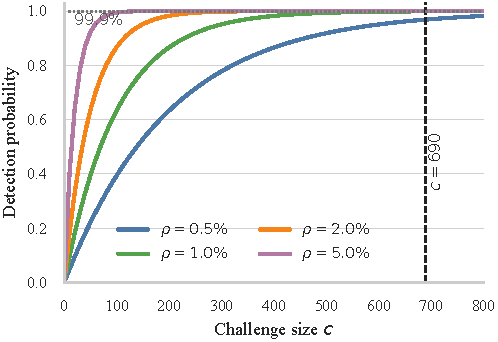
\includegraphics[width=0.43\textwidth]{figures/attack_simulation/sampling_detection_probability.pdf}
\caption{Detection probability with challenge size \(c\).}
\label{fig:sampling_detection_probability}
\end{figure}

\begin{theorem}[Privacy against Honest-but-Curious Verifier]\label{thm:privacy}
Under Assumptions~\ref{ass:random_oracle} and~\ref{ass:discrete_log}, suppose every mask $\mu_i$ is freshly sampled from $\FF_p$ and each challenged evaluation $y_i=f_i(r_i)$ has entropy of at least $\kappa$-bits. Then an honest-but-curious verifier that performs at most $q$ tests recovers $y_i$ with probability at most $q2^{-\kappa}+\mathsf{negl}(\lambda)$. Recovering raw sectors $\{m_{i,j,k}\}$ from the remaining group commitments requires solving discrete logarithms or learning the trapdoor $\tau$.
\end{theorem}

\begin{proof}
The value $\tilde{y}_i=y_i+\mu_i$ is one-time padded by the fresh uniform mask $\mu_i$. The public commitment \(R_i=g^{\mu_i}\), however, makes low-entropy evaluations vulnerable to offline candidate testing: for a guessed value \(y'\), the verifier can check whether \(R_i=g^{\tilde{y}_i-y'}\). Under the stated entropy condition, \(q\) such tests identify \(y_i\) with probability at most \(q2^{-\kappa}\).

For values outside the tested candidate set, recovering \(\mu_i\) from \(R_i=g^{\mu_i}\) requires solving a discrete logarithm in \(\GG_1\), except with negligible probability. Likewise, recovering raw sector coefficients from \(\sigma_{i,j}\), \(b_i\), or \(C_{w_i}\) would require solving discrete logarithms or learning the trapdoor \(\tau\). Thus the transcript hides challenged evaluations only under the stated entropy condition and hides raw sectors under the discrete-log and KZG setup assumptions.
\end{proof}



\subsection{Complexity Analysis}
\label{sec:complexity_analysis}
We measure computational overhead in terms of group exponentiations ($\CompExp$) and bilinear pairings ($\CompPair$). 
Dominant proof-generation finite-field additions and multiplications are reported separately in Table~\ref{tab:computation}. Hash-to-group calls in the source are implemented as base scalar multiplications and are counted as one $\CompExp$ each. In the \textsf{Store} phase, the DO knows the SRS trapdoor and computes each KZG tag as a direct base exponentiation \(g^{f(\tau)}\), costing one \(\CompExp\). When the CS or verifier computes a KZG-style commitment from the public SRS, we count the scalar multiplication for each committed coefficient. Communication overhead is measured in bits using $|p|$, $|\GG_1|$, and $|h|$ for a field element, a $\GG_1$ element, and a hash digest, respectively.

\paragraph{Computation Complexity.} 
\begin{itemize}
    \item $\Store$ Algorithm. In the implementation, the DO knows \(\tau\) during storage and computes each tag directly as \(\sigma_{i,j}=g^{f_{i,j}(\tau)}\). Field evaluation of \(f_{i,j}(\tau)\) is omitted under the metric, and the group work is one base exponentiation per tag. Across $m$ files and $n$ chunks, the storage-side group cost is
    $mn\CompExp.$
    \item $\ProofGen$ Algorithm. For each file, after forming the aggregated polynomial $f_i(X)=\sum_{k=0}^{s-1}a_{i,k}X^k$ in the field, the CS computes the aggregate commitment as $b_i=g^{f_i(\tau)}=\prod_{k=0}^{s-1}(g^{\tau^k})^{a_{i,k}}$ using the SRS. This costs $s\CompExp$, rather than $c\CompExp$, and is equivalent to $\prod_{j\in J}\sigma_{i,j}^{v_{i,j}}$ by the homomorphism of KZG commitments. The CS also computes the mask commitment $R_i=g^{\mu_i}$ using $\CompExp$, the quotient commitment $C_{w_i}=g^{w_i(\tau)}$ using $(s-1)\CompExp$, and the Schnorr commitment $A_i=g^{a_i}$ using $\CompExp$. Thus proof generation costs $= ms\CompExp+m\CompExp+m(s-1)\CompExp+m\CompExp = (2ms+m)\CompExp.$
    
    The additional finite-field work comes from aggregating the $c$ challenged chunk polynomials, evaluating $f_i(r_i)$, and computing the linear quotient. This polynomial work contributes the \(\mathcal{O}(mcs\CompField)\) term shown in Table~\ref{tab:computation}. Since the audit challenge size satisfies $c>s$ in the intended parameter regime, computing $b_i$ from the coefficient vector of $f_i$ keeps proof generation at $\mathcal{O}(ms\CompExp)$ rather than $\mathcal{O}(mc\CompExp)$, while the source-executed runtime still includes polynomial-aggregation work.
    \item $\Verify$ Algorithm. The verifier recomputes $\hat b_i=\prod_{j\in J}\sigma_{i,j}^{v_{i,j}}$ for all files using $mc\CompExp$. It verifies the Schnorr mask proofs using $2m\CompExp$, constructs the folded accumulators $L=\prod_i(b_iR_ig^{-\tilde{y}_i}C_{w_i}^{r_i})^{\rho^{i-1}}$ and $R=\prod_iC_{w_i}^{\rho^{i-1}}$ using $4m\CompExp$, and checks one two-pairing equation. Therefore verification costs $(mc+6m)\CompExp+2\CompPair.$
\end{itemize}

\paragraph{Communication Complexity.}
FoldAudit reduces the expensive algebraic verification to one folded pairing equation, but the audit proof itself is not constant-size in the batch size $m$ or challenge size $c$. The transcript intentionally carries per-file masking and quotient commitments, challenged tags, and Merkle authentication paths so that tag membership and aggregation can be checked explicitly.


\begin{itemize}
    \item $\Store$ Algorithm. The DO transmits raw file data to the CS, incurring $mns|p|$ bits. Concurrently, $mn$ homomorphic tags $\{\sigma_{i,j}\}$ are outsourced to enable future homomorphic aggregation, costing $mn|\GG_1|$ bits. The DO securely shares $m$ Merkle root hashes $\{\Gamma_i\}_{i=1}^m$ with the verifier for audit authentication, requiring $m|h|$ bits. The total one-time outsourcing communication is $mns|p| + mn|\GG_1| + m|h|$.
    % \[
    % \begin{aligned}
    % \underbrace{mns|p|}_{\text{File data}}+
    % \underbrace{mn|\GG_1|}_{\text{Tags}}+
    % \underbrace{m|h|}_{\text{Merkle roots}}=mns|p|+mn|\GG_1|+m|h| .
    % \end{aligned}
    % \]
    \item $\ProofGen$ Algorithm. For each file $i\in[m]$, the proof contains $c$ challenged tags $\{\sigma_{i,j}\}_{j\in J}$, three group elements $(R_i,C_{w_i},b_i)$, one field element $\tilde{y}_i$, one Schnorr commitment $A_i$, one Schnorr response $z_i$, and $c$ Merkle authentication paths. Therefore the total proof communication is $m(c+4)|\GG_1|+2m|p|+mc\log_2 n|h|.$
    
\end{itemize}






\subsection{Dynamic File Management}
Dynamic support is a central requirement in practical PDP systems~\cite{Erway2009DPDP,Wang2011TPDS,Yang2013TPDS,XuTIFS26}. In many outsourced-storage services, files are added and deleted much more frequently than audit rounds are executed: a user may update the active dataset continuously, while the auditor checks integrity hourly, daily, or according to a compliance schedule. FoldAudit natively supports this setting through independent per-file KZG commitments and modular Merkle trees. Crucially, $\ProofGen$ and $\Verify$ are stateless per audit round; they operate on the current active file set without maintaining persistent or incremental proof state. Dynamic operations thus only affect the $\Store$ phase and metadata synchronization.


When the DO uploads a new file $F_{m+1}$, it encodes each chunk into $f_{m+1,j}(X)$, computes tags $\sigma_{m+1,j}=g^{f_{m+1,j}(\tau)}$, and constructs a fresh Merkle tree yielding root $\Gamma_{m+1}$. The data and tags are outsourced to the CS, while $\Gamma_{m+1}$ is securely shared with the verifier. The active batch size increments to $m \leftarrow m+1$. No existing file tag, Merkle root, quotient witness, or global accumulator is recomputed. At the next scheduled audit, $F_{m+1}$ is automatically incorporated through the expanded active file identifier set and Merkle root set.


To remove $F_{i_{\text{del}}}$ from subsequent audits, the DO and V revoke $\Gamma_{i_{\text{del}}}$ from the active metadata set and exclude the corresponding file identifier from future challenges. The CS may reclaim the associated data, tags, and Merkle nodes according to the storage policy, but this protocol action is only an audit-set update and does not prove physical erasure. Surviving files simply skip the removed identifier in subsequent audit loops, incurring zero recomputation of tags or Merkle roots. The active batch size decreases by one, and future $\ProofGen$ executions simply iterate over the reduced active set.

\textit{Complexity of Dynamic Operations.} Adding a single file requires $\mathcal{O}(n\CompExp)$ time for tag generation, as implied by the \textsf{Store} algorithm under the DO-known trapdoor computation. Removing a file from the active audit set only updates the metadata registry and requires no tag generation, Merkle reconstruction for surviving files, SRS regeneration, trapdoor rotation, or global commitment recomputation. Since proof generation is challenge-driven and stateless, dynamic updates incur overhead strictly at the storage and metadata layers. Consequently, the \textsf{ProofGen} and \textsf{Verify} algorithms retain the same complexity as analyzed in Section~\ref{sec:complexity_analysis}.

\begin{table*}[!t]
  \centering
  \caption{Functional and Security Feature Comparison with Related Works}
  \label{tab:feature_comparison_simplified}
  \renewcommand{\arraystretch}{1.12}
  \begin{tabular}{l|c|c|c|c|c}
    \hline
    \textbf{Scheme} & \textbf{Multi-File Batch} & \textbf{Independent $r_i$} & \textbf{Evaluation Privacy} & \textbf{Dynamic Ops.} & \textbf{Cancellation Resistance} \\
    \hline
    Xu et al.~\cite{XuTIFS26} (TIFS26) & \cmark & \xmark & \xmark & \cmark$^\ast$ & \xmark \\
    Zhang et al.~\cite{ZhangTPDS23} (TPDS23) & \cmark & \cmark & \xmark & \xmark & \xmark \\
    Yu et al.~\cite{YuTC25} (TC25) & \xmark & -- & \xmark$^\dag$ & \cmark$^\ast$ & -- \\
    Miao et al.~\cite{MiaoSCIS2026} (SCIS26) & \cmark & -- & \cmark & \cmark & \xmark \\
    \textbf{FoldAudit} & \cmark & \cmark & \cmark & \cmark & \cmark \\
    \hline
  \end{tabular}
  \vspace{0.5mm}
  \footnotesize
  \begin{tabular}{p{0.96\textwidth}}
    $-$: not applicable.
    $\dag$: The privacy-enhanced variant of Yu et al.~\cite{YuTC25} masks only the constant term by $\beta\eta$; its disclosed quotient polynomial can leak non-constant data-polynomial coefficients under repeated audits.
    % $\ddag$: Miao et al.~\cite{MiaoSCIS2026} audit keyword-matched files in aggregate rather than arbitrary polynomial openings.
    $\ast$: Yu et al.~\cite{YuTC25} and Xu et al.~\cite{XuTIFS26} support chunk/block-level updates.
  \end{tabular}
\end{table*}

\begin{table*}[!t]
\centering
\caption{Computational Complexity Comparison (Exponentiations $\CompExp$ and Pairings $\CompPair$) in Multi-File Setting}
\label{tab:computation}
\renewcommand{\arraystretch}{1.3}
\begin{tabular}{l|c|c|c}
\hline
\textbf{Scheme} & \textbf{$\Store$} & \textbf{$\ProofGen$} & \textbf{$\Verify$} \\
\hline
Xu et al.~\cite{XuTIFS26} (TIFS26) & $mn\CompExp$ & $m(s-1)\CompExp+\mathcal{O}(mcs\CompField)$ & $(mc+2)\CompExp+2\CompPair$ \\
Zhang et al.~\cite{ZhangTPDS23} (TPDS23) & $3mn\CompExp$& $(mc+m+2s-2)\CompExp+\mathcal{O}((mcs+m^2s)\CompField)$& $(3mc+m+3)\CompExp+4\CompPair$\\
Yu et al.~\cite{YuTC25} (TC25) & $mn\CompExp$ & $m\CompExp+\mathcal{O}(mcs\CompField)$ & $m(c+2s+1)\CompExp$\\
Miao et al.~\cite{MiaoSCIS2026} (SCIS26) &  $(m\ell+2m+3mn)\CompExp$ & $(mc+1)\CompExp+\mathcal{O}(mc\CompField)$ & $(2mc+m+2)\CompExp+2\CompPair$\\
\hline
\textbf{FoldAudit} & $mn\CompExp$ & $(2ms+m)\CompExp+\mathcal{O}(mcs\CompField)$ & $(mc+6m)\CompExp+2\CompPair$ \\
\hline
\end{tabular}
\vspace{1mm}
\footnotesize
\begin{minipage}{0.96\textwidth}
\(\CompField\) appears only in \textsf{ProofGen} and denotes one modular addition or multiplication over \(\FF_p\) in polynomial aggregation, evaluation, and quotient computation; it excludes inversion, exponentiation, hashing, scalar decoding, and group operations. The \(mcs\)-scaled terms mainly affect Yu et al.~\cite{YuTC25}, Xu et al.~\cite{XuTIFS26}, and FoldAudit; Zhang et al.~\cite{ZhangTPDS23} leverage PCS for multiple points and polynomials (PCS-MPAP)~\cite{Boneh2020PCS}, whereas Miao et al.~\cite{MiaoSCIS2026} have only \(\mathcal{O}(mc\CompField)\).
\end{minipage}
\end{table*}

\begin{table*}[!t]
\centering
\caption{Communication Complexity Comparison (in bits) in Multi-File Setting}
\label{tab:communication}
\renewcommand{\arraystretch}{1.3}
\begin{tabular}{l|c|c}
\hline
\textbf{Scheme} & \textbf{$\Store$ Phase} & \textbf{$\ProofGen$ Phase} \\
\hline
Xu et al.~\cite{XuTIFS26} (TIFS26) & $mns|p|+mn|\GG_1|+m|h|$& $m\bigl(|p|+(c+1)|\GG_1|+c\log_2 n|h|\bigr)$\\
Zhang et al.~\cite{ZhangTPDS23} (TPDS23) & $mns|p| + mn|\GG_1|$& $3|\GG_1| + |p|$\\
Yu et al.~\cite{YuTC25} (TC25) & $mns|p| + mn|\GG_1| + m|h|$& $m\big((s+1)|p| + (c+1)|\GG_1| + c\log_2 n|h|\big)$\\
Miao et al.~\cite{MiaoSCIS2026} (SCIS26) & $mn|p|+(mn+m)|\GG_1|$ & $|p|+2|\GG_1|$ \\
\hline
\textbf{FoldAudit} & $mns|p| + mn|\GG_1| + m|h|$& $m(c+4)|\GG_1|+2m|p|+mc\log_2 n|h|$ \\
\hline
\end{tabular}
\end{table*}

\section{Related Works}
\label{sec:related_works}

The foundational PDP model of Ateniese et al.~\cite{Ateniese2007PDP} introduces probabilistic possession checks with compact authenticators.
The generation of authentication tags can be realized in several ways. Early PDP constructions use RSA-based homomorphic tags, where the algebraic structure of the tag allows multiple challenged blocks to be combined into one compact proof \cite{Ateniese2007PDP}. Symmetric-key variants based on message authentication codes (MACs) provide lower computational overhead, but they usually support only private verification and are less suitable for third-party auditing~\cite{Ateniese2008Scalable}.


Ateniese et al.'s basic PDP model~\cite{Ateniese2007PDP} is RSA-based and mainly targets static outsourced data, and it does not naturally support efficient insertions, deletions, or modifications. To address this limitation, dynamic PDP schemes support block updates while preserving auditability, often by combining authenticated data structures with PDP-style proofs~\cite{Ateniese2008Scalable,Erway2009DPDP,Duan2023DecentralizedAudit}. Another important line of work is publicly verifiable PDP, where verification can be delegated to an external auditor without revealing the data owner's secret key~\cite{Wang2011TPDS,Shu2022BlockchainAudit,Wang2014TCC,Chen2024ObjectAuditing,Chen2024ServerlessAuditing}. 
Such schemes typically rely on public-key homomorphic authenticators, including BLS signature-based constructions, so that a third-party auditor can check storage correctness on behalf of the client \cite{Shacham2008POR,Wang2013TC,Liu2025TLARDA}. 


Polynomial and vector commitments are a useful toolkit for making storage-auditing proofs compact. KZG commitments~\cite{Kate2010KZG} provide constant-size commitments and pairing-based openings for low-degree polynomials, while vector commitments~\cite{Catalano2013VC,Campanelli20ASIACRYPT} and accumulators~\cite{Boneh2019Batching} offer a way to authenticate large indexed data with short update or membership evidence. Du et al.~\cite{Du22TDSC} bring this idea into decentralized storage auditing by using KZG commitments as blockchain-assisted metadata: instead of publishing bulky block-level evidence, the audit can bind many data blocks to succinct on-chain proof material and keep public verification lightweight. The same pressure toward short audit evidence also appears in dynamic cold storage~\cite{Yu2024EDCOMA}.
Campanelli et al.~\cite{Campanelli20ASIACRYPT} introduce incrementally aggregatable vector commitments with subvector openings in hidden-order groups, enabling compact openings to be generated and combined in decentralized storage.



Xu et al.~\cite{XuTIFS26} propose MPA, a lightweight and updatable auditing scheme that combines polynomial commitments with Merkle authentication for decentralized multi-copy storage. MPA supports full aggregation across files and providers and uses a blockchain-assisted procedure to derive unpredictable challenges. However, the multi-file verification equation aggregates all local proofs at a shared evaluation point $r$. Therefore, the batch check does not provide independent per-file evaluation points or an explicit random-folding soundness bound for cross-file cancellation.
% it verifies a globally aggregated opening together with Merkle membership paths.

Zhang et al.~\cite{ZhangTPDS23} address on-chain overhead for decentralized multi-copy auditing by instantiating the PCS-MPAP batch polynomial commitment. 
Their batch scheme assigns distinct evaluation points $\{r_l\}_{l=1}^d$ to files and publishes a constant-size per-storage-service-provider (per-SSP) proof $(\sigma'_i,W_i,W'_i,E_i)$.
This construction substantially reduces on-chain storage and avoids linear growth in the number of files. Nevertheless, the batch proof exposes an unmasked linear combination \(E_i=\sum_{l=1}^d\beta_lS_{l,i}\), where \(S_{l,i}=F_{l,M_i}(r_l)=\sum_{(a_j,v_j)\in Q_l}v_jf_{l,m_i,a_j}(r_l)\). Since the challenge transcript publishes $\{\beta_l,r_l,Q_l\}$, each audit round reveals a public linear equation in the challenged block-polynomial coefficients. Across repeated audits with linearly independent challenge vectors, these equations can be accumulated to recover evaluation values and, eventually, the underlying data-polynomial coefficients for repeatedly challenged blocks. Thus, Zhang et al.~\cite{ZhangTPDS23} do not provide evaluation privacy against an honest-but-curious verifier or public observer. 

Yu et al.~\cite{YuTC25} design a storage verification scheme for resource-constrained Industrial Internet of Things (IIoT) environments. It combines a homomorphic hash function, polynomial commitments, and a tag-indexed Merkle hash tree (Tag-IMHT) authenticated structure to eliminate pairings from verification and to support chunk-level modification, insertion, and deletion. Its privacy-enhanced variant adds a random constant term $\beta\eta$ to the proof polynomial and returns an additional masking tag $B$. However, the proof still discloses the quotient polynomial $Z_{\mathrm{prf}}(x)=(P_{\mathrm{prf}}(x)-P_{\mathrm{prf}}(z))/(x-z)$. Since the constant mask cancels in this quotient, $Z_{\mathrm{prf}}(x)$ reveals the non-constant coefficients of the challenged aggregate polynomial; repeated audits with different challenge coefficients may therefore leak the underlying data polynomial, while only the constant term is protected by $\beta\eta$. The scheme also does not provide a native multi-file batch verification equation; auditing multiple files requires independent protocol executions.

Recently, Miao et al.~\cite{MiaoSCIS2026} propose a blockchain-assisted multi-keyword searchable PDP scheme. Its index matrix and match indexes let the verifier check that all files matching the queried keywords participate in the audit, thereby addressing search-result integrity, pre-matching, and pre-computation attacks. The proof $\{T,\mu_1,R\}$ aggregates authenticators over the matched files and masks the aggregate data value as $\mu_1=\mu-rh_1(T_w,R)$. Thus, Miao et al.~\cite{MiaoSCIS2026} support keyword-filtered multi-file auditing and data privacy. 






Table~\ref{tab:feature_comparison_simplified} compares the features of related works.
Tables~\ref{tab:computation} and~\ref{tab:communication} summarize the source-aligned comparison. We use \(m\) for the number of files in one audit batch, \(n\) for chunks per file, \(s\) for sectors per chunk, and \(c\) for challenged chunks per file; for Miao et al.~\cite{MiaoSCIS2026}, \(\ell\) is the average number of keywords attached to each file. The computation table counts expensive group exponentiations \(\CompExp\) and pairings \(\CompPair\), while dominant proof-generation finite-field additions and multiplications are shown only in the \textsf{ProofGen} column. Hash-to-group calls implemented as base scalar multiplications are counted as one \(\CompExp\); group additions, PRF calls, byte hashes, Merkle-path hashing, searchable-index row decryption, field inversion, field exponentiation, hash-to-scalar conversion, and auxiliary metadata outside \((m,n,s,c,\ell)\) are omitted from the main count.
% The tables follow the system-level reproductions under \texttt{schemes/}. Yu et al.~\cite{YuTC25} are counted as independent multi-file audits because their scheme has no native cross-file batch equation; Zhang et al.~\cite{ZhangTPDS23} and Xu et al.~\cite{XuTIFS26} are normalized to the single-replica/provider case \(N=1\); and Miao et al.~\cite{MiaoSCIS2026} use \(m\) for the number of keyword-matched files. Store-phase KZG tags are counted from the data-owner side, where the trapdoor is known and each tag costs one base exponentiation; public-SRS commitments computed by the server or verifier count one scalar multiplication per committed coefficient. 
Appendix~\ref{app:complexity_derivations} derives Tables~\ref{tab:computation} and~\ref{tab:communication}, while FoldAudit's row is derived in Section~\ref{sec:complexity_analysis}.








\section{Evaluation}
\label{sec:evaluation}

\subsection{Experimental Environment and Parameter Setting}

All experiments were conducted on a local Apple M4 machine with 10 logical CPU cores and 16~GB of memory, running macOS~26.3. The host hardware reports the \texttt{arm64} architecture, while the Go toolchain used for the benchmark binary reports \texttt{darwin/amd64}. The implementation was compiled and executed with Go~1.25.4. Pairing and group operations were instantiated with the \texttt{bn256} curve. Each compared protocol was reproduced under the same Go framework with its system-level audit path: storage/tag generation, challenge derivation, proof generation, and verification are implemented for multi-file audit tests.
For cross-checking only, Table~\ref{tab:primitive_latency} reports the
single-operation latencies measured on the same backend.
The result tests that hash-to-group (i.e., \textsf{HashToG1}) costs nearly the same with $\CompExp$. The source codes are available on Github\footnote{\url{https://github.com/scottocs/foldaudit}}.

\begin{table}[h]
\centering
\caption{Operation Latency for Cross-Checking Only}
\label{tab:primitive_latency}
\renewcommand{\arraystretch}{1.2}
\begin{tabular}{l|c}
\hline
\textbf{Operation} & \textbf{Latency ($\mu$s/op)} \\
\hline
Finite-field add/mul over \(\FF_p\) (\(\ComField\)) & 0.410 \\
\(\GG_1\) addition (omitted in Table~\ref{tab:computation}) & 0.415 \\
\(\GG_1\) scalar multiplication (\(\CompExp\)) & 70.168 \\
\(\GG_2\) scalar multiplication (\(\CompExp'\)) & 345.117 \\
\textsf{HashToG1} (counted as \(\CompExp\)) & 70.928 \\
Pairing check term (\(\CompPair\)) & 1153.475 \\
\hline
\end{tabular}
\end{table}



We first demonstrate that related works suffer from data leakage and cancellation attack, as summarized by Table~\ref{tab:feature_comparison_simplified}. Fig.~\ref{fig:attack_bound_illustrations} reports the corresponding attack simulations. Fig.~\ref{fig:data_leakage_attack_cost} converts the number of repeated audit transcripts needed for linear recovery into measured attack cost; Yu et al.~\cite{YuTC25} exhibits partial leakage, Xu et al.~\cite{XuTIFS26} and Zhang et al.~\cite{ZhangTPDS23} expose recoverable unmasked equations, while Miao et al.~\cite{MiaoSCIS2026} and FoldAudit avoid this direct leakage model through fresh masking. Fig.~\ref{fig:cancellation_attack_cost} evaluates cancellation-forgery attempts under fixed \(m=4\), \(n=64\), \(s=8\), and \(c=8\): Zhang et al.~\cite{ZhangTPDS23}, Miao et al.~\cite{MiaoSCIS2026}, and Xu et al.~\cite{XuTIFS26} accept the constructed cancellations, whereas Yu et al.~\cite{YuTC25} and FoldAudit reject them.



\begin{figure}[h]
\centering
\subfloat[Leakage attack cost.]{

\includegraphics[width=0.45\textwidth]{figures/attack_simulation/data_leakage_attack_cost.pdf}
\label{fig:data_leakage_attack_cost}}
\\[0.6ex]
\subfloat[Cancellation attack cost.]{

\includegraphics[width=0.45\textwidth]{figures/attack_simulation/cancellation_attack_cost.pdf}
\label{fig:cancellation_attack_cost}}
\caption{Data leakage attack and cancellation attack for repeated-data auditing.}
\label{fig:attack_bound_illustrations}
\end{figure}




\begin{figure*}[!t]
\centering
\subfloat[Store vs. file size.]{

\includegraphics[width=0.31\textwidth]{figures/vi_evaluation/store_vs_file_size.pdf}
\label{fig:store_vs_file_size}}
\hfill
\subfloat[Store vs. sectors.]{
\includegraphics[width=0.31\textwidth]{figures/vi_evaluation/store_vs_s.pdf}
\label{fig:store_vs_s}}
\hfill
\subfloat[Store vs. batch size.]{
\includegraphics[width=0.31\textwidth]{figures/vi_evaluation/store_vs_m.pdf}
\label{fig:store_vs_m}}

\subfloat[ProofGen vs. file size.]{
\includegraphics[width=0.31\textwidth]{figures/vi_evaluation/proofgen_vs_file_size.pdf}
\label{fig:proofgen_vs_file_size}}
\hfill
\subfloat[ProofGen vs. sectors.]{

\includegraphics[width=0.31\textwidth]{figures/vi_evaluation/proofgen_vs_s.pdf}
\label{fig:proofgen_vs_s}}
\hfill
\subfloat[ProofGen vs. batch size.]{
\includegraphics[width=0.31\textwidth]{figures/vi_evaluation/proofgen_vs_m.pdf}
\label{fig:proofgen_vs_m}}

\subfloat[Verify vs. file size.]{
\includegraphics[width=0.31\textwidth]{figures/vi_evaluation/verify_vs_file_size.pdf}
\label{fig:verify_vs_file_size}}
\hfill
\subfloat[Verify vs. sectors.]{

\includegraphics[width=0.31\textwidth]{figures/vi_evaluation/verify_vs_s.pdf}
\label{fig:verify_vs_s}}
\hfill
\subfloat[Verify vs. batch size.]{
\includegraphics[width=0.31\textwidth]{figures/vi_evaluation/verify_vs_m.pdf}
\label{fig:verify_vs_m}}
\caption{Runtime under different parameter setting. When varying \(B\), we fix \(m=4\), \(s=20\), and \(c=690\); when varying \(s\), we fix \(m=4\), \(B=10\)~MB, and \(c=690\); when varying \(m\), we fix \(B=10\)~MB, \(s=20\), and \(c=690\).}
\label{fig:vi_runtime_sweeps}
\end{figure*}


The evaluation fixes the challenge size at $c=690$, following the parameter choice in Remark~\ref{rem:parameter_selection}, and varies three workload dimensions.
% The batch size $m$ ranges over $\{4,8,12,16,20\}$, the file size $B$ ranges over $\{10,20,30,40,50\}$~MB, and the number of sectors per chunk $s$ ranges over $\{20,40,60,80,100\}$. 
The baseline setting is $m=4$, $B=10$~MB, and $s=20$. 
% We use a one-factor-at-a-time evaluation: when varying $B$, we fix $m=4$ and $s=20$; when varying $s$, we fix $m=4$ and $B=10$~MB; when varying $m$, we fix $B=10$~MB and $s=20$. Each workload point is executed ten times, and the reported value is the median. The standard deviation across the ten executions is retained in the generated CSV files. 
The number of chunks per file $n$ is not treated as an independent parameter. Since each sector is represented by one field element of approximately $|p|=256$ bits, one encoded chunk contains $32s$ bytes; therefore, for a file of size $B$ bytes, we set \(n=\max\{c,\lceil B/(32s)\rceil\}\). 
% The lower bound $n\geq c$ is required because the challenge set samples $c$ distinct chunks from $[n]$. When the raw size-derived value $\lceil B/(32s)\rceil$ is smaller than $c$, the encoded file representation is padded to $c$ chunks so that the sampling rule remains well-defined.
We choose $s<c$ throughout the experiments. 
% This is not merely a formatting choice: $s$ determines the degree bound of each chunk polynomial and the SRS length, whereas $c$ determines how many chunks are sampled in one audit. FoldAudit first aggregates the $c$ challenged chunks of each file into an $s$-coefficient polynomial and then computes the KZG witness over this degree-$(s-1)$ object. 
% Keeping $s<c$ ensures that this compression is meaningful and that proof generation is governed by $\mathcal{O}(ms\CompExp)$ for the witness-related exponentiations rather than by a larger per-challenge polynomial dimension. 
If $s\geq c$, the intended advantage of compressing many challenged chunks into a lower-degree per-file aggregate is weakened and the SRS, commitment, and witness costs increase without improving the detection probability, which is already controlled by $c$.


\subsection{Performance Results}

To evaluate the computational behavior under the above parameter setting, we execute each implemented scheme end-to-end on simulated file contents. 


Fig.~\ref{fig:store_vs_file_size} reports the storage-generation cost as the file size grows under direct source execution. This phase is dominated by tag generation over all encoded chunks and therefore grows with $mn$. FoldAudit has the same asymptotic storage-generation cost $\mathcal{O}(mn\CompExp)$ as Yu et al.~\cite{YuTC25} and Xu et al.~\cite{XuTIFS26} under the DO-known trapdoor computation. Zhang et al.~\cite{ZhangTPDS23} and Miao et al.~\cite{MiaoSCIS2026} require additional group/hash-to-curve work during tag construction, so their setup cost is higher under the same backend. 

Fig.~\ref{fig:proofgen_vs_s} evaluates the effect of the number of sectors per chunk. Since $c$ is fixed at $690$, increasing $s$ enlarges the per-chunk polynomial representation and the field aggregation work in \textsf{ProofGen}. FoldAudit scales approximately linearly in $s$ for witness-related group operations, matching the complexity $(2ms+m)\CompExp$ in Table~\ref{tab:computation}. Miao et al. scheme~\cite{MiaoSCIS2026} is included in this figure only as a non-SRS baseline under the same file-parsing workload; $s$ is not its native SRS degree parameter, and its \textsf{ProofGen} complexity is essentially independent of $s$. 
% In the measured range, FoldAudit's proof-generation time increases from $0.1000$~s at $s=20$ to $0.4966$~s at $s=100$; it remains below Zhang et al.~\cite{ZhangTPDS23} but above Yu et al.~\cite{YuTC25}, Xu et al.~\cite{XuTIFS26}, and the nearly flat Miao et al.~\cite{MiaoSCIS2026} proof-generation path at larger $s$.

Figs.~\ref{fig:verify_vs_file_size}, \ref{fig:verify_vs_s}, and~\ref{fig:verify_vs_m} show that verification is almost insensitive to file size and the sector count, while it grows with the batch size because each additional file contributes challenged-tag aggregation and per-file proof terms. FoldAudit preserves the intended verifier-side compactness: once the server has compressed the challenged sectors into folded polynomial commitments and witnesses, the verifier checks a folded equation with two pairings and $\mathcal{O}(mc)$ group operations.

Fig.~\ref{fig:proof_communication_vs_m} complements the runtime measurements with audit-proof communication costs derived in Table~\ref{tab:communication}. Zhang et al.~\cite{ZhangTPDS23} and Miao et al.~\cite{MiaoSCIS2026} have constant-size proof transcripts, whereas Yu et al.~\cite{YuTC25}, Xu et al.~\cite{XuTIFS26}, and FoldAudit grow linearly in \(m\) because they explicitly include challenged tags and Merkle authentication paths. 
FoldAudit pays a modest additional per-file cost for masking and folded KZG consistency material, but remains in the same communication order as Merkle-authenticated sampled-tag designs. 
% Overall, FoldAudit is not the absolute minimum in raw local computation or proof size, but it stays within the same order as the fastest Merkle-authenticated schemes while providing multi-file folded verification, evaluation masking, and explicit sampled-tag authentication.

\begin{figure}[h]
\centering
\subfloat[Storage communication (with fixed \(m=4\), \(s=20\))]{

\includegraphics[width=0.45\textwidth]{figures/vi_evaluation/store_communication_vs_file_size.pdf}
\label{fig:store_communication_vs_file_size}}
% \end{figure}
% \begin{figure}[h]
\\[0.6ex]
\subfloat[Proof communication (with fixed \(B=10\)~MB, \(s=20\), and \(c=690\))]{

\includegraphics[width=0.45\textwidth]{figures/vi_evaluation/proof_communication_vs_m.pdf}
\label{fig:proof_communication_vs_m}}
\vspace{-0.6em}
\caption{Communication overhead of the one-shot $\Store$ algorithm and each $\ProofGen$ algorithm execution.}
\label{fig:vi_aggregate_overhead}
\end{figure}

\noindent\textbf{Deployment Implications for Lightweight Devices.}
Similar to recent cloud-assisted IIoT storage verification scenarios~\cite{YuTC25}, FoldAudit is also particularly well-suited for deployment in resource-constrained environments. 
Its design minimizes on-device computational and storage overhead by offloading heavy cryptographic operations—such as batch proof generation and polynomial evaluations—to the cloud server, while keeping the verifier-side logic compact and efficient. Specifically, the verifier only performs a constant number of pairing operations and lightweight hash-based checks, which aligns well with the limited processing capabilities of lightweight devices. Moreover, the use of homomorphic aggregation and folded verification significantly reduces communication bandwidth, an important factor for edge and IoT settings with constrained network resources. The incorporation of Merkle-authenticated tags further ensures that devices only need to store succinct root metadata instead of full datasets. FoldAudit's algebraic folding and masking mechanisms enable privacy-preserving audits with minimal local workload. Therefore, the protocol achieves a favorable balance between security and efficiency, making it practical for large-scale deployment across lightweight devices in industrial IoT and edge computing scenarios where energy, computation, and storage are tightly limited.

% Despite these advances, existing schemes leave at least one of the following gaps: no native arbitrary multi-file batch audit, no independent per-file polynomial challenge points, limited evaluation privacy on transparent ledgers, susceptibility to cross-file cancellation in aggregated checks, or dynamic support with a different update granularity. FoldAudit addresses these gaps through Fiat--Shamir folding over independently challenged per-file quotient equations, transcript-bound masked evaluations, and stateless file addition and active audit-set removal; its folded-relation analysis separately quantifies the residual algebraic cancellation probability.

\section{Conclusion}

This paper presented FoldAudit, a dynamic multi-file PDP protocol that provides sound and efficient integrity auditing for outsourced storage. By combining per-file KZG commitments, Merkle-authenticated sampled tags, independent evaluation points, additive one-time masking, and Fiat--Shamir folding, FoldAudit enables multiple files to be audited through a single folded verification relation while preserving per-file accountability. The design avoids structurally coupled openings and prevents cross-file cancellation by ensuring that each file contributes an independently bound quotient relation before folding. It also protects challenged evaluations from honest-but-curious verifiers through fresh masks and Schnorr proofs, while retaining compatibility with public verification.
We formally prove that the folded verification relation has negligible soundness error. FoldAudit further supports stateless file addition and active audit-set removal without rebuilding commitments for unaffected files. Our implementation and comparisons show that FoldAudit achieves competitive audit overhead across different file sizes, sector counts, and batch sizes. Although storage initialization remains the dominant one-time cost, the results demonstrate that FoldAudit is practical for scalable, privacy-preserving, and cancellation-resistant multi-file auditing.



\begin{thebibliography}{00}


\bibitem{Shah2007Auditing}
M.~A.~Shah, M.~Baker, J.~C.~Mogul, and R.~Swaminathan,
``Auditing to keep online storage services honest,''
in \emph{HotOS}, 2007, pp.~1--6.

\bibitem{Sookhak2015Survey}
M.~Sookhak, A.~Gani, M.~K.~Khan, and R.~Buyya,
``Remote data auditing in cloud computing environments: A survey, taxonomy, and open issues,''
\emph{ACM Comp. Surv.}, vol.~47, no.~4, article~65, pp.~1--34, 2015.

\bibitem{Deswarte2004RIC}
Y.~Deswarte, J.-J.~Quisquater, and A.~Sa{\"i}dane,
``Remote integrity checking,''
in \emph{Integrity and Internal Control in Information Systems VI}, 2004, pp.~1--11.

\bibitem{Schwarz2006Store}
T.~J.~E. Schwarz and E.~L.~Miller,
``Store, forget, and check: Using algebraic signatures to check remotely administered storage,''
in \emph{ICDCS}, 2006, pp.~12--12.

\bibitem{Ateniese2007PDP}
G.~Ateniese, R.~Burns, R.~Curtmola, J.~Herring, L.~Kissner, Z.~Peterson, and D.~Song,
``Provable data possession at untrusted stores,''
in \emph{ACM CCS}, 2007, pp.~598--609.

\bibitem{Bowers2009HAIL}
K.~D.~Bowers, A.~Juels, and A.~Oprea,
``HAIL: A high-availability and integrity layer for cloud storage,''
in \emph{CCS}, 2009, pp.~187--198.

\bibitem{Stefanov2012Iris}
E.~Stefanov, M.~van Dijk, A.~Juels, and A.~Oprea,
``Iris: A scalable cloud file system with efficient integrity checks,''
in \emph{ACSAC}, 2012, pp.~229--238.

\bibitem{Ateniese2011RDC}
G.~Ateniese, R.~Burns, R.~Curtmola, J.~Herring, O.~Khan, L.~Kissner, Z.~Peterson, and D.~Song,
``Remote data checking using provable data possession,''
\emph{ACM Transactions on Information and System Security}, vol.~14, no.~1, article~12, pp.~1--34, 2011.

% \bibitem{Curtmola2008MRPDP}
% R.~Curtmola, O.~Khan, R.~Burns, and G.~Ateniese,
% ``MR-PDP: Multiple-replica provable data possession,''
% in \emph{ICDCS}, 2008, pp.~411--420.

\bibitem{Juels2007POR}
A.~Juels and B.~S.~Kaliski Jr.,
``PORs: Proofs of retrievability for large files,''
in \emph{ACM CCS}, 2007, pp.~584--597.

\bibitem{Le2023Porla}
T.~Le, P.~Huang, A.~A. Yavuz, E.~Shi, and T.~Hoang,
``Efficient dynamic proof of retrievability for cold storage,''
in \emph{NDSS}, 2023.

\bibitem{Kate2010KZG}Kate, A., Zaverucha, G.M. and Goldberg, I. Constant-size commitments to polynomials and their applications. In \emph{Asiacrypt}, 2010, pp. 177-194.

\bibitem{Boneh2020PCS}Boneh, D., Drake, J., Fisch, B. and Gabizon, A. Efficient polynomial commitment schemes for multiple points and polynomials. Cryptology ePrint Archive. 2020.

\bibitem{YuTC25}
H.~Yu, H.~Zhang, Z.~Yang, Y.~Chen, and H.~Liu,
``Efficient and Secure Storage Verification in Cloud-Assisted Industrial IoT Networks,''
\emph{IEEE TC}, vol.~74, no.~5, pp.~1702--1716, 2025.

\bibitem{ZhangTPDS23}
Q.~Zhang, Z.~Zhang, J.~Cui, H.~Zhong, Y.~Li, C.~Gu, and D.~He,
``Efficient Blockchain-Based Data Integrity Auditing for Multi-Copy in Decentralized Storage,''
\emph{IEEE TPDS}, vol.~34, no.~12, pp.~3162--3172, 2023.

\bibitem{Dumas2023VESPo}
J.-G.~Dumas, A.~Maignan, C.~Pernet, and D.~S. Roche,
``VESPo: Verified evaluation of secret polynomials with application to dynamic proofs of retrievability,''
\emph{PET}, vol.~2023, no.~4, pp.~766--791, 2023.

\bibitem{Yu2024EDASVIC}
H.~Yu, H.~Zhang, Z.~Yang, and S.~Yu,
``EDASVIC: Enabling efficient and dynamic storage verification for clouds of industrial internet platforms,''
\emph{IEEE TIFS}, vol.~19, pp.~6896--6909, 2024.

\bibitem{XuTIFS26}
Y.~Xu, H.~Cheng, J.~Zheng, X.~Zhang, and H.~Wang,
``MPA: Lightweight and Updatable Integrity Auditing for Decentralized Storage Using Merkle Trees and Polynomial Commitments,''
\emph{IEEE TIFS}, vol.~21, pp.~2162--2176, 2026.

\bibitem{Shu2022BlockchainAudit}
J.~Shu, X.~Zou, X.~Jia, W.~Zhang, and R.~Xie,
``Blockchain-based decentralized public auditing for cloud storage,''
\emph{IEEE TCC}, vol.~10, no.~4, pp.~2366--2380, 2022.

\bibitem{Cui2024PayPerProof}
H.~Cui, Z.~Wan, T.~Zhaolu, H.~Wang, and A.~Miyaji,
``Pay-per-proof: Decentralized outsourced multi-user PoR for cloud storage payment using blockchain,''
\emph{IEEE Transactions on Cloud Computing}, vol.~12, no.~1, pp.~130--144, 2024.

\bibitem{Xu2024BDACD}
Y.~Xu, C.~Jin, W.~Qin, J.~Zhao, G.~Chen, and F.~Zeng,
``BDACD: Blockchain-based decentralized auditing supporting ciphertext deduplication,''
\emph{JSA}, vol.~147, article~103053, 2024.

\bibitem{MiaoSCIS2026}
Y.~Miao, K.~K.~Gai, and L.~Zhu,
``Blockchain-Assisted Multi-Keyword Searchable Provable Data Possession for Cloud Storage,''
\emph{SCIS}, vol.~69, no.~3, article~132101, 2026.

\bibitem{Ateniese2008Scalable}
G.~Ateniese, R.~Di Pietro, L.~V.~Mancini, and G.~Tsudik,
``Scalable and efficient provable data possession,''
in \emph{SecureComm}, 2008, pp.~1--10.

\bibitem{Shacham2008POR} H.~Shacham and B.~Waters,
``Compact proofs of retrievability,''
in \emph{ASIACRYPT}, 2008, pp.~90--107.

\bibitem{Dodis2009POR}
Y.~Dodis, S.~Vadhan, and D.~Wichs,
``Proofs of retrievability via hardness amplification,''
in \emph{TCC}, pp.~109--127, 2009.

\bibitem{Wang2010PrivacyAudit}
C.~Wang, Q.~Wang, K.~Ren, and W.~Lou,
``Privacy-preserving public auditing for data storage security in cloud computing,''
in \emph{INFOCOM}, 2010, pp.~1--9.

\bibitem{Wang2013TC}
C.~Wang, S.~S.~M.~Chow, Q.~Wang, K.~Ren, and W.~Lou,
``Privacy-preserving public auditing for secure cloud storage,''
\emph{IEEE TC}, vol.~62, no.~2, pp.~362--375, 2013.

% \bibitem{Zhu2012TPDS}
% Y.~Zhu, H.~Hu, G.-J.~Ahn, and M.~Yu,
% ``Cooperative provable data possession for integrity verification in multicloud storage,''
% \emph{IEEE TPDS}, vol.~23, no.~12, pp.~2231--2244, 2012.

\bibitem{Schnorr1991Sig}C.P. Schnorr. Efficient signature generation by smart cards. \emph{JoC}, 4(3), pp.161-174, 1991.

\bibitem{Erway2009DPDP}
C.~Erway, A.~K{\"u}p{\c{c}}{\"u}, C.~Papamanthou, and R.~Tamassia,
``Dynamic provable data possession,''
in \emph{CCS}, 2009, pp.~213--222.

\bibitem{Wang2011TPDS}
Q.~Wang, C.~Wang, J.~Li, K.~Ren, and W.~Lou,
``Enabling public verifiability and data dynamics for storage security in cloud computing,''
\emph{IEEE TPDS}, vol.~22, no.~5, pp.~847--859, 2011.

\bibitem{Yang2013TPDS}
K.~Yang and X.~Jia,
``An efficient and secure dynamic auditing protocol for data storage in cloud computing,''
\emph{IEEE TPDS}, vol.~24, no.~9, pp.~1717--1726, 2013.

\bibitem{Duan2023DecentralizedAudit}
H.~Duan, Y.~Du, L.~Zheng, C.~Wang, M.~H. Au, and Q.~Wang,
``Towards practical auditing of dynamic data in decentralized storage,''
\emph{IEEE TDSC}, vol.~20, no.~1, pp.~708--723, 2023.

\bibitem{Wang2014TCC}
B.~Wang, B.~Li, and H.~Li,
``Oruta: Privacy-preserving public auditing for shared data in the cloud,''
\emph{IEEE TCC}, vol.~2, no.~1, pp.~43--56, 2014.

% \bibitem{Yu2017TIFS}
% Y.~Yu, M.~H.~Au, G.~Ateniese, X.~Huang, W.~Susilo, Y.~Dai, and G.~Min,
% ``Identity-based remote data integrity checking with perfect data privacy preserving for cloud storage,''
% \emph{IEEE TIFS}, vol.~12, no.~4, pp.~767--778, 2017.

\bibitem{Chen2024ObjectAuditing}
F.~Chen, F.~Meng, Z.~Li, L.~Li, and T.~Xiang,
``Public cloud object storage auditing: Design, implementation, and analysis,''
\emph{JPDC}, vol.~188, article~104870, 2024.

\bibitem{Chen2024ServerlessAuditing}
F.~Chen, J.~Cai, T.~Xiang, and X.~Liao,
``Practical cloud storage auditing using serverless computing,''
\emph{SCIS}, vol.~67, no.~3, 2024.

\bibitem{Liu2025TLARDA}
K.~Liu, J.~Ning, P.~Wu, S.~Xu, and R.~Chen,
``TLARDA: Threshold label-aggregating remote data auditing in decentralized environment,''
\emph{IEEE TIFS}, vol.~20, pp.~3146--3160, 2025.

\bibitem{Catalano2013VC}
D.~Catalano and D.~Fiore,
``Vector Commitments and Their Applications,''
in \emph{PKC}, pp.~55--72, 2013.

\bibitem{Campanelli20ASIACRYPT}
M.~Campanelli, D.~Fiore, N.~Greco, D.~Kolonelos, and L.~Nizzardo,
``Incrementally Aggregatable Vector Commitments and Applications to Verifiable Decentralized Storage,''
in \emph{ASIACRYPT}, pp.~3--35, 2020.

\bibitem{Boneh2019Batching}
D.~Boneh, B.~B{\"u}nz, and B.~Fisch,
``Batching techniques for accumulators with applications to IOPs and stateless blockchains,''
in \emph{CRYPTO}, 2019, pp.~561--586.

\bibitem{Du22TDSC}
Y.~Du, H.~Duan, A.~Zhou, C.~Wang, M.~H.~Au, and Q.~Wang,
``Enabling Secure and Efficient Decentralized Storage Auditing with Blockchain,''
\emph{IEEE TDSC}, vol.~19, no.~5, pp.~3038--3054, 2022.

% \bibitem{Guo2019ODPDP}
% W.~Guo, H.~Zhang, S.-J.~Qin, F.~Gao, Z.~Jin, W.~Li, and Q.~Wen,
% ``Outsourced dynamic provable data possession with batch update for secure cloud storage,''
% \emph{Future Generation Computer Systems}, vol.~95, pp.~309--322, 2019.

\bibitem{Yu2024EDCOMA}
H.~Yu, Y.~Chen, Z.~Yang, Y.~Chen, and S.~Yu,
``EDCOMA: Enabling efficient double compressed auditing for blockchain-based decentralized storage,''
\emph{IEEE TSC}, vol.~17, no.~5, pp.~2273--2286, 2024.

\end{thebibliography}

\begin{IEEEbiography}[{\includegraphics[width=1in,height=1.25in,clip,keepaspectratio]{liangzhang}}]{Liang Zhang} was born in 1989. He received a bachelor's degree in computer science from Huazhong University of Science and Technology, Wuhan, in 2012. After five years of being an engineer in the IT industry, he joined Fudan University in 2017 and acquired his Ph.D. degree in 2022. He became an associate professor at Hainan University in 2024 and he is currently a research assistant professor in The Hong Kong University of Science and Technology. His research interests include Web 3.0, blockchain and applied cryptography. His recent publications are included in \emph{IEEE TC}, \emph{IEEE TIFS}, \emph{IEEE TMC}, \emph{IEEE TSC}, \emph{IEEE TBD}, \emph{CJ}, \emph{CSCWD'25}, \emph{APWEB'23}, \emph{CF'22} and \emph{SACMAT'22}.
\end{IEEEbiography}

\begin{IEEEbiography}[{\includegraphics[width=1in,height=1.25in,clip,keepaspectratio]{xuyanwei.eps}}]{Xuyan Wei}
obtained a Bachelor’s degree in Computer Science and Technology and is currently pursuing a Master’s degree in Cybersecurity at the School of Cyberspace Security, Hainan University. Her research interests include blockchain applications, provable data possession and related security technologies.
\end{IEEEbiography}


\begin{IEEEbiography}[{\includegraphics[width=1in,height=1.25in,clip,keepaspectratio]{boruichen.eps}}]{Borui Chen}
obtained Bachelor's degree in Computer Science from Fudan University in 2023 and is currently pursuing a Master's degree in Cyberspace Security at the same university. His research interests include zero-knowledge proof, blockchain and attribute-based encryption.
\end{IEEEbiography}



\begin{IEEEbiography}[{\includegraphics[width=1in,height=1.25in,clip,keepaspectratio]{haibinkan}}]{Haibin Kan} was born in 1971. He received a Ph.D. from Fudan University, Shanghai, China, 1999. From June 2002 to February 2006, he was with the Japan Advanced Institute of Science and Technology as an assistant professor. He went back Fudan University in February 2006, where he is currently a full professor. He is also the Director of the Shanghai Blockchain Engineering Research Center. His research interests include coding theory, cryptography, and computation complexity. 
\end{IEEEbiography}

\begin{IEEEbiography}[{\includegraphics[width=1in,height=1.25in,clip,keepaspectratio]{jiheng.eps}}]{Jiheng Zhang} joined IEDA as an Assistant Professor in 2009, and was promoted to Associate Professor in 2015 and then to full Professor in 2020. His research interests are in the areas of service operations management, queueing system and applied probability. He is an outstanding scholar in the field of Stochastic Modelling and Optimization, Statistical Learning, Numerical Methods and Algorithm, as evidenced by publishing ten papers in leading journals of his discipline since his substantiation, including Management Science, Operations Research, and Mathematics of Operations Research. He has been serving as Associate Editor for Operations Research, Stochastic Systems, and Queueing Models and Service Management, and an editorial board member for Probability in the Engineering and Informational Sciences. 
\end{IEEEbiography}
\vfill


\appendix
\subsection{Complexity Derivations for Compared Schemes}
\label{app:complexity_derivations}
\noindent
This appendix derives the non-FoldAudit rows of Tables~\ref{tab:computation} and~\ref{tab:communication}; FoldAudit is derived in Section~\ref{sec:complexity_analysis}. Table~\ref{tab:feature_comparison_simplified} is qualitative and is supported by the scheme discussion and attack simulations.

\noindent\textit{a.1) Computation Complexity of Yu et al.~\cite{YuTC25} (TC25)}
\begin{itemize}
\item \textbf{$\Store$ Algorithm.}  In the source, the DO knows the setup trapdoor \(\psi\) and computes each chunk tag directly as \(g^{f(\psi)}\). Therefore, each tag costs \(\CompExp\), and the storage computation for $m$ independent files is \(mn\CompExp\).
\item \textbf{$\ProofGen$ Algorithm.} The only counted group exponentiation is the privacy mask \(B=g^\beta\). In addition, each independent file constructs the challenged aggregate polynomial and its quotient, adding \(\mathcal{O}(mcs\CompField)\) finite-field additions and multiplications. Therefore, over \(m\) independent files, the Table~\ref{tab:computation} entry is \(m\CompExp+\mathcal{O}(mcs\CompField)\).
\item \textbf{$\Verify$ Algorithm.}  For each file, the verifier aggregates the \(c\) challenged tags, computes \(B^\eta\), commits the quotient polynomial through \texttt{CommitG1}, computes the shifted quotient commitment loop in the source, and forms the terms \(H_Z^{-z}\) and \(g^{P_{\mathrm{prf}}(z)}\). Since the quotient has at most \(s-1\) coefficients, this costs \((c+2s+1)\CompExp\) per independent audit. Thus, auditing \(m\) files independently costs \(m(c+2s+1)\CompExp\).
\end{itemize}

\noindent\textit{a.2) Communication Complexity of Yu et al.~\cite{YuTC25} (TC25)}
\begin{itemize}
\item \textbf{$\Store$ Algorithm.} The data owner uploads \(mns\) field sectors and \(mn\) homomorphic tags to the server, and shares one Merkle root per file with the verifier. Hence the one-time storage communication is \(mns|p|+mn|\GG_1|+m|h|\).
\item \textbf{$\ProofGen$ Algorithm.}  For each file, the response contains the quotient polynomial, one evaluation value, \(c\) challenged tags, one mask \(B\), and \(c\) Merkle paths of length $\log n$. Since the quotient has \(s-1\) field coefficients, the value plus quotient contributes \(s|p|\). Across \(m\) files, the proof communication is \(m(s+1)|p|+m(c+1)|\GG_1|+mc\log n|h|\).
\end{itemize}

\noindent\textit{b.1) Computation Complexity of Zhang et al.~\cite{ZhangTPDS23} (TPDS23)}
\begin{itemize}
\item \textbf{$\Store$ Algorithm.}  For each file block, the source derives \(H(F_{id}\|i\|j)\) through \texttt{HashToG1Bytes}, computes \(g^{f_{i,j}(\alpha)}\) directly using the DO-known trapdoor \(\alpha\), and then applies the outer secret-key power. Counting the hash-to-group derivation as one exponentiation, this gives \(3\CompExp\) per tag and \(3mn\CompExp\) in total.
\item \textbf{$\ProofGen$ Algorithm.} For each file, exponentiating the \(c\) challenged tags by their audit coefficients costs \(c\CompExp\), and applying the file-folding coefficient \(\beta_l\) costs one more exponentiation. Since the storage server does not know the SRS trapdoor \(\alpha\), the source computes \(W\) and \(W'\) as KZG commitments over the public SRS: \(W=\mathsf{Commit}(H_b)\) and \(W'=\mathsf{Commit}(L(X)/(X-z))\). Both committed polynomials have at most \(s-1\) coefficients, contributing \(2(s-1)\CompExp\). Polynomial aggregation and PCS-MPAP batch-polynomial construction add \(\mathcal{O}((mcs+m^2s)\CompField)\) finite-field additions and multiplications. Therefore, the Table~\ref{tab:computation} entry is \((mc+m+2s-2)\CompExp+\mathcal{O}((mcs+m^2s)\CompField)\).
\item \textbf{$\Verify$ Algorithm.} The verifier constructs \(\zeta\) by deriving each hashed index through \texttt{HashToG1Bytes}, exponentiating it by its audit coefficient, and then exponentiating the intermediate term by the corresponding folding coefficient in the nested source loop. This costs \((3mc+m)\CompExp\). It also forms \(\psi=g^{-E_1}\cdot W_1^{-Z_T(z)}\) and \(u\cdot v^{-z}\), which contributes \(3\CompExp\).  The batch equation \(e(\sigma',g)e(\psi,v)=e(\zeta,v)e(W',u\cdot v^{-z})\) contains four pairings. Hence, verification costs \((3mc+m+3)\CompExp+4\CompPair\).
\end{itemize}

\noindent\textit{b.2) Communication Complexity of Zhang et al.~\cite{ZhangTPDS23} (TPDS23)}
\begin{itemize}
\item \textbf{$\Store$ Algorithm.}  The storage phase sends the file copy, containing \(mns\) field sectors, and \(mn\) tags. The storage communication is \(mns|p|+mn|\GG_1|\).
\item \textbf{$\ProofGen$ Algorithm.}  The published proof is \((\sigma',W_1,W'_1,E_1)\), namely three group elements and one field element. Therefore the audit-proof communication is \(3|\GG_1|+|p|\).
\end{itemize}

\noindent\textit{c.1) Computation Complexity of Miao et al.~\cite{MiaoSCIS2026} (SCIS26)}
\begin{itemize}
\item \textbf{$\Store$ Algorithm.}  In IndexGen, the data owner computes \(H_{F_i}\) from the file keywords, derives \(H_2(FID_i)\), and computes one match index \(\Omega_i=(H_{F_i}\cdot H_2(FID_i))^{-x}\) per file. With \(\ell\) keywords per file on average, this costs \(m\ell\CompExp+m\CompExp+m\CompExp\). In AuthGen, the data owner creates one authenticator \(\sigma_{i,j}=(H_{F_i}\cdot H_2(FID_i)\cdot H_3(au_{i,j})\cdot u^{m_{i,j}})^x\) for each block. In the source, each block authenticator derives \(H_3(au_{i,j})\), performs \(u^{m_{i,j}}\), and applies the outer secret-key exponentiation. This contributes \(3mn\CompExp\). Therefore the full storage-side computation is \((m\ell+2m+3mn)\CompExp\), with no pairing.
\item \textbf{$\ProofGen$ Algorithm.}  After locating the matched set of \(m\) files, the server computes \(T=\prod_{i\in R}\prod_{j\in Q}\sigma_{i,j}^{e_{i,j}}\), which costs \(mc\CompExp\), and generates the privacy element \(R_g=g^r\), which costs one more exponentiation. The aggregate data value \(\mu\) adds \(\mathcal{O}(mc\CompField)\) finite-field additions and multiplications. Thus the Table~\ref{tab:computation} entry is \((mc+1)\CompExp+\mathcal{O}(mc\CompField)\).
\item \textbf{$\Verify$ Algorithm.}  The verifier exponentiates one match index \(\Omega_i\) for each matched file. For each challenged block, it derives the \(H_3(au_{i,j})\) term through hash-to-group and exponentiates that term by the audit coefficient. It also computes \(u^{\mu_1}\) and \(R_g^{h_1(T_w,R_g)}\). These operations contribute \((m+2mc+2)\CompExp\). The final verification equation has two pairings, so the verifier computation is \((2mc+m+2)\CompExp+2\CompPair\).
\end{itemize}

\noindent\textit{c.2) Communication Complexity of Miao et al.~\cite{MiaoSCIS2026} (SCIS26)}
\begin{itemize}
\item \textbf{$\Store$ Algorithm.}  The data and authenticators sent to the cloud contribute \(mn|p|+mn|\GG_1|\). The match indexes contain one group element per file, adding \(m|\GG_1|\). Thus the normalized storage communication is \(mn|p|+(mn+m)|\GG_1|\), excluding auxiliary searchable index metadata such as addresses and encrypted index matrices.
\item \textbf{$\ProofGen$ Algorithm.}  The audit proof \((T,\mu_1,R_g)\) consists of two group elements and one field element, so the proof communication is \(|p|+2|\GG_1|\).
\end{itemize}

\noindent\textit{d.1) Computation Complexity of Xu et al.~\cite{XuTIFS26} (TIFS26)}
\begin{itemize}
\item \textbf{$\Store$ Algorithm.}  For each file and block, the data owner forms the block polynomial and computes the tag \(\sigma_{i,j}=g^{f_{m_{i,j}}(\alpha)}\). Since the DO knows \(\alpha\), tag generation costs one base exponentiation for each of the \(mn\) tags. Hashing the Merkle leaves and roots is omitted under the current computation metric. The storage-side \textsf{TagVerify} cost reported by Xu et al.~\cite{XuTIFS26} is a separate validation phase and is not included in this Store column. Thus the normalized storage computation is \(mn\CompExp\), with no pairing.
\item \textbf{$\ProofGen$ Algorithm.}  For each file, the CS linearly combines the \(c\) challenged block polynomials, evaluates the aggregate polynomial at the challenge point, and divides by \(X-r\). These finite-field and polynomial operations add \(\mathcal{O}(mcs\CompField)\). The counted group operation is the KZG witness \(w_i=g^{h_i(\alpha)}\). Since \(h_i(X)\) has degree at most \(s-2\), computing the witness from the structured public key costs \((s-1)\CompExp\) per local proof. Across \(m\) local proofs, the Table~\ref{tab:computation} entry is \(m(s-1)\CompExp+\mathcal{O}(mcs\CompField)\), with no pairing.
\item \textbf{$\Verify$ Algorithm.}  The verifier first aggregates the challenged tags by computing \(\prod_{j=1}^{c}\sigma_{i,a_j}^{v_j}\) for every file, which costs \(mc\CompExp\). It then computes \(g^{val^{global}}\) and \(g^{\alpha-r}\), adding \(2\CompExp\). The accepted batch path checks one global KZG equation, requiring the two pairings \(\hat e(\sigma^{global}/g^{val^{global}},g)\) and \(\hat e(w^{global},g^{\alpha-r})\). Thus verification costs \((mc+2)\CompExp+2\CompPair\). The fallback diagnosis used only after a failed global check is not included in this normal verification cost.
\end{itemize}

\noindent\textit{d.2) Communication Complexity of Xu et al.~\cite{XuTIFS26} (TIFS26)}
\begin{itemize}
\item \textbf{$\Store$ Algorithm.}  The source stores \(mn\) encrypted blocks, each with \(s\) field sectors, and \(mn\) polynomial tags. The Merkle root for each file is published as the verification anchor. It does not transmit a Merkle path for every stored block in the storage-phase interface. Therefore the one-time storage communication is \(mns|p|+mn|\GG_1|+m|h|\).
\item \textbf{$\ProofGen$ Algorithm.}  For each file, the proof contains one evaluation value \(val_i\), one witness \(w_i\), the \(c\) challenged tags, and \(c\) Merkle authentication paths. Across \(m\) proofs, the audit-proof communication is \(m\bigl(|p|+(c+1)|\GG_1|+c\log_2 n|h|\bigr)\).
\end{itemize}

\vfill


\end{document}
